\documentclass[aps,pre,twocolumn,showpacs,showkeys,superscriptaddress,floatfix]{revtex4-1}
 %\pdfoutput=1 \input epsf

\usepackage[utf8]{inputenc}
\usepackage[english]{babel}
\usepackage{hyperref}

\usepackage{amsmath}
\usepackage{amssymb}
\usepackage{amscd}
\usepackage{mathtools}

\usepackage{color}
\usepackage{graphicx}
\usepackage{subfigure}

\usepackage{upgreek}
\usepackage{dcolumn}
\usepackage{natbib}

\DeclareMathOperator{\erfc}{erfc}

\newcommand{\rmd}{{\mathrm d}}
\newcommand{\rme}{{\mathrm e}}
\newcommand{\dbar}{{\mathchar '26 \mkern-11mu {\mathrm d}}}

\renewcommand{\vec}[1]{{\boldsymbol {#1}}}
 %  \usepackage{showkeys}

\begin{document} 

\title{The interaction between Actin and Myosin-II, the flashing ratchet}
\author{Pieter Baerts}
%\author{Christian Maes}
\affiliation{KU Leuven, Instituut voor Theoretishe Fysica, Celestijnenlaan 200D, B-3001 Leuven, Belgium}
\author{Jiří Pešek}
\author{Herman Ramon}
\affiliation{KU Leuven, BIOSYST-MeBioS, Kasteelpark Arenberg 30, B-3001 Leuven, Belgium}

\begin{abstract}
Recent advancements in experimental methods has demonstrated that molecular motors from the Myosin~II family are not only driving the cytoskeleton, 
but more importantly they serve as cross-links inducing an active tension in the network. 
Here we revise the Brownian ratchet model, 
which was previously studied in the context of an active transport, 
in setups resembling a motor placed in a polymer network.
We show that such a model is not only capable of capturing mechanosensing behavior,
but also its chemical cycle's efficiency is directly related to the active tension on the motor.  
\end{abstract}

\maketitle 

\section{Introduction}

The cytoskeleton of a cell mainly consists of long semi-flexible actin polymers and myosin II molecular motors\cite{mitchison1996actin}. 
These motors contain several heads that are able to bind to polymer filaments and walk along them\cite{pollard1982structure}. 
The mechanism for walking relies both on a chemical cycle in the motor's head and on the asymmetry of a periodic and electrostatic potential along the length of such a polymer\cite{Reimann2002introduction}. 
The cytoskeleton serves two main purposes, being transporting large vesicles and governing the cell's motility, i.e. the ability of the cell to move and change its shape \cite{ross2008cargo,mitchison1996actin}.
The part of the cytoskeleton that plays a crucial role in the motility of the cell is the actin-myosin cortex \cite{vicente2009non} and it will serve as the exemplary system in this paper.

In recent research, it has been argued that the role of myosin~II motors is mainly to generate tension in the actin polymer network\cite{ma2012nonmuscle,chugh2017actin,monier2010actomyosin}.
Therefore, the main goal of this work is to introduce an efficiency of the motor that is not related to transport, but rather to tension in the motor.
We show that this efficiency is directly related to the net supply of energy provided by the chemical cycle 
and we investigate how this chemical efficiency depends on ATP concentrations and on external force on the system.
However, before we do so, we revisit certain features of molecular motors in a simple Brownian ratchet model\cite{reimann2002brownian} with constant chemical rates and relate the force-velocity relation to the mean force generated by the ratchet and to tension in the motor.

The chemical cycle that powers the molecular motor is driven by ATP molecules that can attach to a head of the motor, causing it to change the charge of the head and consequently loosen its bond with the polymer filament \cite{adelstein1980regulation}. 
When bound to a motor head, the ATP molecule will hydrolyze to ADP and release a phosphate\cite{gajewski1986thermodynamics}. 
It this state, the head can attach to the polymer again, ADP will be released from the motor head and the chemical cycle can start over. 
Hence, the chemical state of a motor head will determine how strongly it can be coupled to a cytoskeletal filament\cite{Nie2014,nie2014conformational}. 


Cytoskeletal polymers exhibit a sequence of monomers that cause a periodical structure\cite{yogurtcu2012mechanochemical}. 
Furthermore, these monomers are polarized, so that when chained together in a polymer, they give rise to an asymmetric, ratchet-like, electrostatic potential along the length of the filament \cite{Nie2014,nie2014conformational}. 
An example of such a potential is shown in figure \ref{fig:energy}. 
The heads of a myosin~II motor, too, carry an electric charge\cite{barterls1993myosin} and therefore they will feel the ratchet potential of the filaments. 
When the chemical state of the head changes, so does its molecular structure and charge. 
As mentioned earlier, this causes the bond between the head and filament to either strengthen or loosen. 
Therefore, the head will experience a ratchet potential that is stochastically flashing in time, changing the amplitude of the potential from high to low.


In the state in which the motor is tightly bound to the filament, the head will most probably be very close to a minimum in the ratchet potential, 
while in the unbound state, it is easier for the motor to diffuse over a larger distance. 
However, because of the asymmetry of the ratchet, the motor will be biased to explore one side of the ratchet rather than the other. 
Therefore, the motor will more likely jump to an adjacent period of the ratchet potential in the preferred direction, indicated by the asymmetry of the ratchet potential \cite{reimann2002brownian}.
This will eventually lead to directed motion of the motor on long timescales\cite{Reimann2002introduction}. 

This mechanism motivates the assumptions of ratchet models, being that the motor heads interact with a periodic asymmetric potential that changes depending on the chemical state of the head. 
Such ratchet models have been studied extensively in the context of molecular motors \cite{reimann2002brownian,astumian1994fluctuation,astumian1996mechanochemical,julicher1997modeling,Reimann2002introduction,julicher1997spontaneous,peskin1995correlation,huxley1969mechanism,huxley1971proposed}.
The models that have been used in these studies are very similar to each other but often differ in some basic assumptions.
The specific model that we have studied is presented in section \ref{sec:ratchet}. 
It has the important trait that the chemical rates do not depend on spacial degrees of freedom and motor heads can attach and detach anywhere along the polymer filament.
Furthermore, the rates do not dependent on external forces on the motor but solely on concentrations of chemicals involved in ATP hydrolysis. We assume that constant concentrations are maintained in the environment at all times. 
The type of motor that we will be studying is non-muscle myosin II, which have a small number of heads \cite{pollard1982structure}. 
These non-muscle myosin~II motors are crucial to the motility of most eukaryotic cells \cite{vicente2009non}.
For larger myosin motors, like the ones in muscle cells, mean-field calculations have led to analytic results for the force-velocity relation \cite{julicher1997modeling}.
In experimental studies with synthetic myosin motors, the number of heads per motor is also much higher than in non-muscle cells. 
Therefore, the results for large motor play a very important role in interpreting and understanding those in-vitro experiments \cite{brown2009cross-correlated}.
For motors with fewer heads, mean-field methods are not suitable and numerical simulations prove to be useful.
In sections \ref{sec:velocity} and \ref{sec:force-velocity} we will describe the dynamics of this motor-polymer system in detail by means of numerical methods.
Furthermore, we investigate the behavior of the motor in various setups, e.g. the coupling of the motor to an elastic environment.
Earlier studies have shown that myosin~II motors are able to sense the stiffness of their environment and that they can adapt the active forces that they generate \cite{stam2015isoforms,albert2014stochastic}.
In those studies the chemical rates did depend on the load on the motor. 
We show that a motor in our simple ratchet model with constant rates behaves similarly.

Another important aspect of molecular motors is their ability to convert chemical energy into mechanical work \cite{astumian1996mechanochemical}.
The chemical cycle of ATP hydrolysis consists out of many consecutive reactions and after one full cycle a net amount of energy is provided to the motor head\cite{gajewski1986thermodynamics}.
However, often this cycle is represented by only two states\cite{julicher1997modeling,Reimann2002introduction}, e.g. ATP bound and ADP bound, 
in which case a stochastic process on these states always satisfies detailed balance and no chemical energy can be extracted. 
In other words, the energetic gain of one reaction is canceled by the cost of the following reaction.
On the other hand, we do not want any redundant degrees of freedom in our description since we are not really interested in the full chemical details of the process.
In section \ref{sec:energie}, we will look at the energy balances in various setups of a myosin~II motor interacting with actin filaments.
A novel way of defining a chemical efficiency, by interpreting the chemical input by measuring the differences in potential energy in each jump, is presented in section \ref{sec:efficiency}.
There, we investigate how this efficiency depends on the external load, number of heads of the motor and ATP concentration. 
We observe that the chemical efficiency is a useful measure, related to the tension in the motor, that is relevant in all of the considered setups.

\section{The Ratchet model}
\label{sec:ratchet}
In order to investigate the movement of myosin along the actin filament and the forces it generates, we consider the following one dimensional model.
At first, we assume that the rigidity of the actin polymer and myosin backbone is high enough that their elongations can be neglected.
Second, we assume that all myosin heads are attached directly to the myosin backbone at fixed equidistant positions, see figure~\ref{fig:ratchet_setup}.
\begin{figure}[t]
\centering
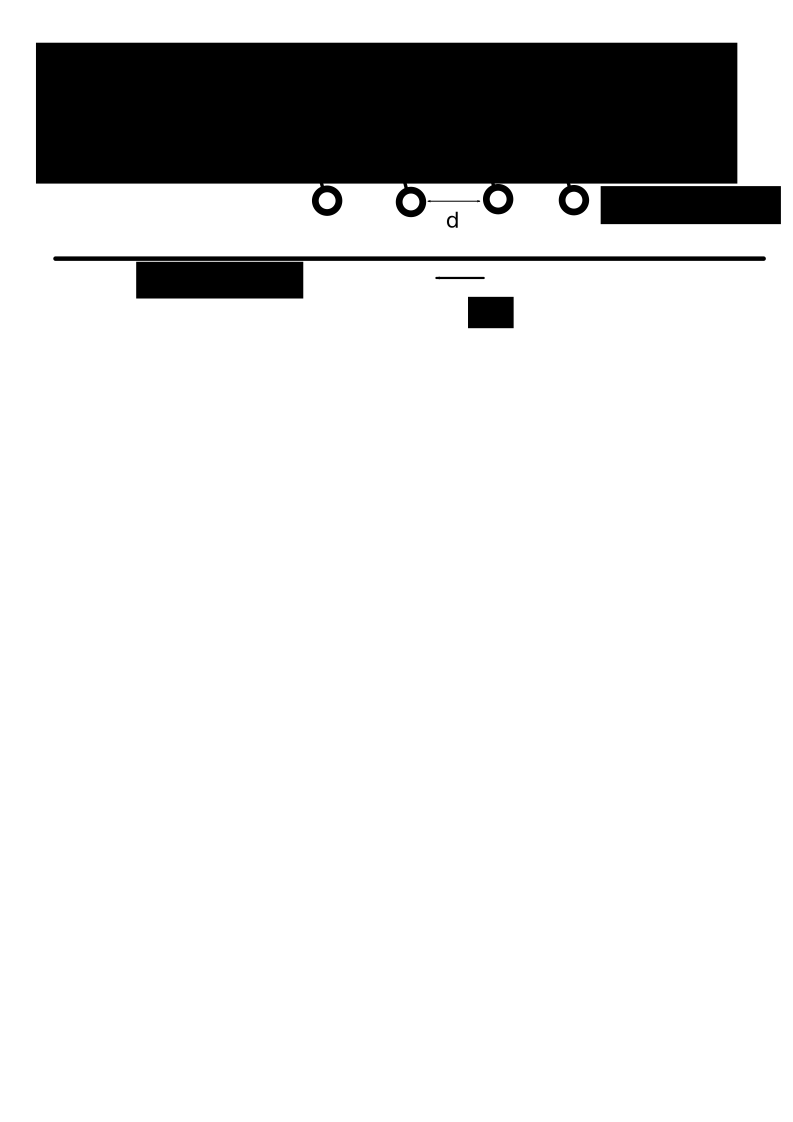
\includegraphics[width=0.45\textwidth,height=!]{ratchet_illustration}
\caption{
\label{fig:ratchet_setup}
In this illustration the basic setup is depicted.  
The backbone of the myosin motor is shown with four heads that are equidistantly spaced with $d$ denoting their respective distance. 
The load $F_\text{load}$ is applied only on myosin and the actin filament is freely diffusing. 
} 
\end{figure}
These simplifications allow us to model both the motor and the filament as point particles undergoing overdamped diffusion in the inter-cellular environment \cite{vanKampen1981stochastic}.
Moreover, each myosin head has an internal state, which represent its chemical state, 
i.e. whether there is an ATP bounded or not to the myosin head. 

The dynamics of positions is described by coupled overdamped Langevin equations 
\begin{align}
&\begin{multlined}[b]
\rmd x_\text{M} = 
- \frac{1}{\gamma_\text{M}} \left[ \nabla_\text{M} V_t(x_\text{M}(t) - x_\text{A}(t)) + F_\text{load} \right] \; \rmd t 
\\ 
+ \sqrt{ \frac{2 k_B T}{\gamma_\text{M}} } \; \rmd W_\text{M} ,
\end{multlined}
\label{eq:eom_M} \\
&\begin{multlined}[b][.42\textwidth]
\rmd x_\text{A} = 
- \frac{1}{\gamma_\text{A}} \nabla_\text{A} V_t(x_\text{M}(t) - x_\text{A}(t)) \; \rmd t 
\\
+ \sqrt{ \frac{2 k_B T}{\gamma_\text{A}} } \; \rmd W_\text{A} ,
\end{multlined}
\label{eq:eom_A}
\end{align}
where $x_\text{M}$ ($x_\text{A}$) denote the position of myosin (actin polymer), 
$\gamma$ is the Stokes drag,
$T$ is the absolute temperature of the environment,
$W$ denotes the Wiener process,
$F_\text{load}$ is an external load on the motor, 
and the interaction potential $V_t$ represents the overall ratchet interaction, which is a sum over individual contributions from all motor heads,
\begin{equation}
V_t(x) = \sum\limits_{i=0}^{N-1} \zeta_t(i) \, V_\text{r} (x - i \, d ), 
\label{eq:ratchet_interaction}
\end{equation}
where $d$ is the distance between myosin heads, 
$N$ is the number of heads per motor,
$\zeta_t(i)$ represents the internal state, see bellow, 
and $V_\text{r}$ is the periodical ratchet potential, see figure~\ref{fig:energy},
\begin{figure}[t]
\centering
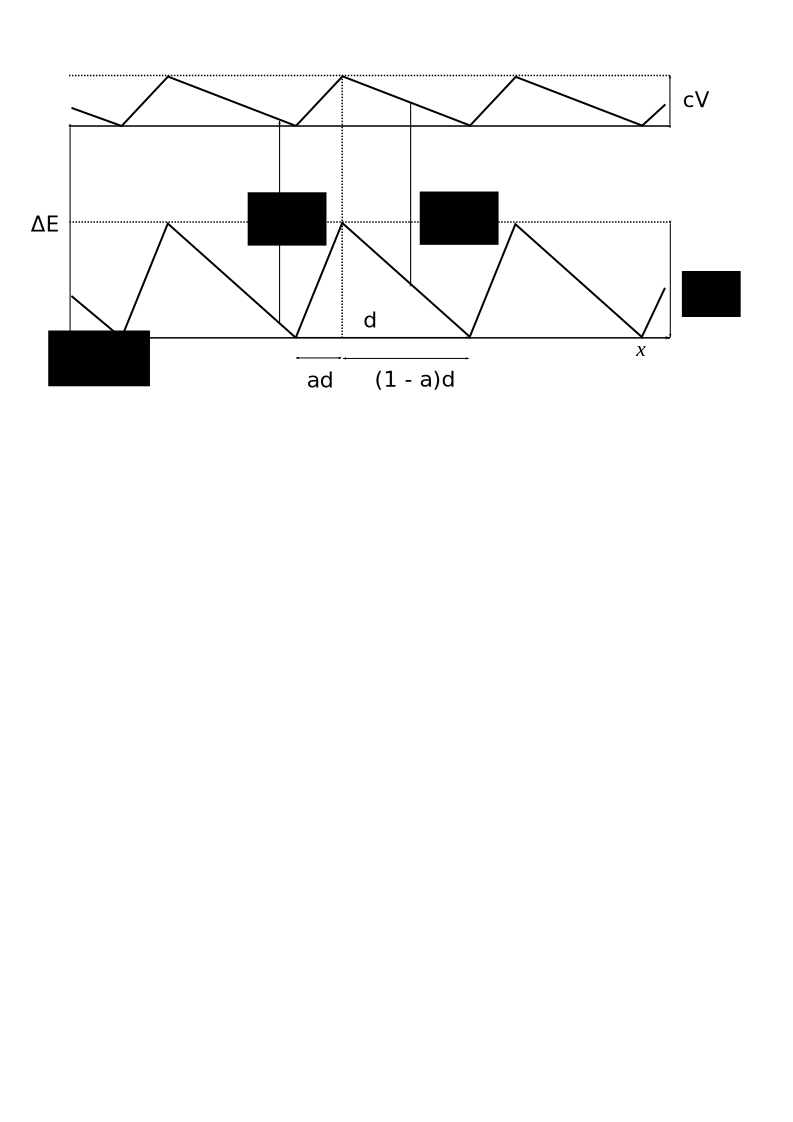
\includegraphics[width=0.45\textwidth,height=!]{energy}
\caption{
\label{fig:energy}
Energy landscape for the myosin's head.
The basic interaction with actin polymer is via Ratchet potential with the potential height $V$, period $\ell$ and skewness parameter $a$.
The transition between ATP \emph{bound} and \emph{unbound} state is govern by rates $k_\text{bind}$, $k_\text{unbind}$ 
and is associated with the chemical energy $\Delta E$.
In the \emph{bound} state the ratchet potential is scaled down by factor $c$. 
}
\end{figure}
\begin{equation}
V_\text{r}(x) =  \begin{cases}
        V_\text{r}(x+\ell) & x < 0 \\[1ex] 
        \displaystyle \frac{ V x }{ a \ell } & 0 \leq x < a \ell \\[2ex]
        \displaystyle \frac{ V (\ell-x) }{ (1-a) \ell } & a \ell \leq x < \ell \\[2ex]
        V_\text{r}(x-\ell) & \ell \leq x  
   \end{cases} ,
   \label{eq:ratchet_potential}
\end{equation}
with total height $V$,
period $\ell$ 
and skewness parameter $a \in [0,1]$. 

The dynamics of the internal state of heads is governed by continuous time Markov process. 
Contrary to other popular choices \cite{}, here the internal state represents whether ATP (or one of its products) is \emph{bound} or \emph{unbound} to the myosin head. %TODO
This specifies the electrostatic properties of the head which will determine the amplitude of the interaction potential with the actin filament.
No effective dependencies on position or external forces are imposed on the dynamics of the chemical cycle. 
Work done by external forces is dissipated through the diffusion processes of the motor and polymer, see section~\ref{sec:energie}.
This is a simplification over the full chemical network governing the internal states of myosin \cite{Bierbaum2011,Bierbaum2013},  
which focuses only on the long lasting states that significantly change the myosin's head physical properties.
Namely, we look at states where ADP is bounded and where there is no molecule bound to myosin head as escape rates from those states are small with respect to other transitions \cite{Bierbaum2011}, %TODO 
for which the estimated free energy landscapes \cite{Nie2014,nie2014conformational} very well reflect the changes in  conformation and electric charge of the myosin head \cite{barterls1993myosin}.
In order to obtain the transition rates between these to two states, we start from the three state model introduced by Albert et al. \cite{albert2014stochastic},
which we further simplify by unifying the state corresponding to the hydrolized ATP (i.e. ADP+P) and ADP with P released state as this process occurs on much shorter time-scale than other transitions.

Lastly, as the internal state reflects the chemical state of the head rather then the act of binding to actin itself,
we assume that external load have little influence on the associated rates but rather opposes the underlying free energy landscape. 
These considerations are reflected in the assumption the rates $k_\text{bind}$, $k_\text{unbind}$ independent of the load, 
but they depend on the concentrations of the relevant chemical species present in ATP hydrolysis. 
More specifically $k_\text{bind}$ is proportional to $[\text{ATP}]$ while $k_\text{unbind}$ is inversely proportional to $[\text{ADP}]$ and $[\text{P}_\text{i}]$.
The dynamics is then represented by dichotomous continuous times Markov process with constant rates,
\begin{equation}
\zeta_t = 1 \overset{k_\text{bind}}{\underset{k_\text{unbind}}{\rightleftarrows}} \zeta_t = c ,
\label{eq:transition}
\end{equation}
where $c\in\left[0,1\right]$ determines the amplitude of the ratchet potential when the motor is loosely bound to the filament, 
which we use as an approximation for changes in the free energy landscape \cite{Nie2014,nie2014conformational}.
While both the diffusion and the jump process are in equilibrium, the mechanism of the flashing ratchet brings the combined system out of equilibrium, leading to the movement of the motor in a preferred direction, given by the asymmetry of the filament \cite{}. %TODO

Figure~\ref{fig:ratchet_setup} depicts the whole setup of the system
and figure~\ref{fig:energy} depicts the dynamics involved in flashing ratchet. 
Table \ref{tab:parameters} lists the values of the parameters used in this model. 
Some of them were taken from the literature while others were fitted to give a realistic mean velocities and stall force for the myosin~II. 
The friction coefficients were calculated with Stokes' law \cite{Broersma1960,Broersma1981}, using the known dimensions of the molecules \cite{yogurtcu2012mechanochemical,pollard1982structure} and the viscosity of the extracellular medium \cite{li2004diffusion}.
\begin{table}[t]
\centering
\begin{ruledtabular}
\begin{tabular}{lcdcc}
Parameter & Symbol & \multicolumn{1}{c}{Value} & Units & Source\\
\hline
Thermal energy& $k_B T$ & 4.28 & pN nm & --- \\
Number of heads& $N$ & 4 & --- & \cite{pollard1982structure}\\
Head's spacing& $l$ & 15 & nm & \cite{pollard1982structure}\\
Step length& $d$ & 8 & nm & \cite{vilfan2003instabilities}\\
Binding rate& $k_\text{unbind}$ & 40 & s$^{-1}$ & \cite{albert2014stochastic} \\
Detaching rate& $k_\text{bind}$ & 80 & s$^{-1}$ & \cite{albert2014stochastic} \\
Skewness& $a$ & 0.25 & --- & ---\\
Potential amplitude& $V$ & 40 & pN nm & ---\\
Potential scaling& $c$ & 0.3 & --- & \cite{Nie2014, nie2014conformational}\\
Chemical energy gap & $\Delta E$ & 30.4 & pN nm & \cite{gajewski1986thermodynamics}\\
Motor friction& $\gamma_{m}$ & 0.66 & pN $\upmu$s nm$^{-1}$ & \cite{Broersma1960,Broersma1981} \\ %TODO
Actin friction& $\gamma_{a}$ & 0.97 & pN $\upmu$s nm$^{-1}$ & \cite{Broersma1960,Broersma1981} \\ %TODO
\end{tabular}
\end{ruledtabular}
\caption{
\label{tab:parameters}
Table of all parameter values and a reference to their source.
}
\end{table}

\subsection{Other setups}
\label{sec:other_setups}
While the aforementioned setup, shown in figure~\ref{fig:ratchet_setup}, is the most studied \cite{reimann2002brownian,astumian1994fluctuation,finer1994single,julicher1997modeling,kishino1988force,peskin1995correlation,saito1994movement},
it's aim is to characterize the transport induced by molecular motors.
However, recent experiments show that myosin~II motors' role is mainly to cross-linking the cytoskeleton 
and consequently producing an active tension inside the network \cite{ma2012nonmuscle}.
Here, we present a couple of natural extensions to this setup, suitable for capturing the behavior of the motor inside these networks.
The basic setup will be further referred to as ``load on the motor''.

\subsubsection{Load on the polymer}
\label{sec:load_on_polymer}
The first setup that we introduce is very similar to ``load on the motor'', 
but now with the external load applied to the polymer instead of the molecular motor. 
This correspond to a situation where the motor is attached to the polymer, which itself is under the tension due to the action of other motors and complex interactions in a larger network.
As we will show later, in this setup there will be no more residual tension on the motor for large loads, which will be relevant for our discussion of the chemical efficiency. 
The basic scheme of this setup is depicted in the figure~\ref{fig:load_on_polymer setup}.
\begin{figure}[t]
\centering
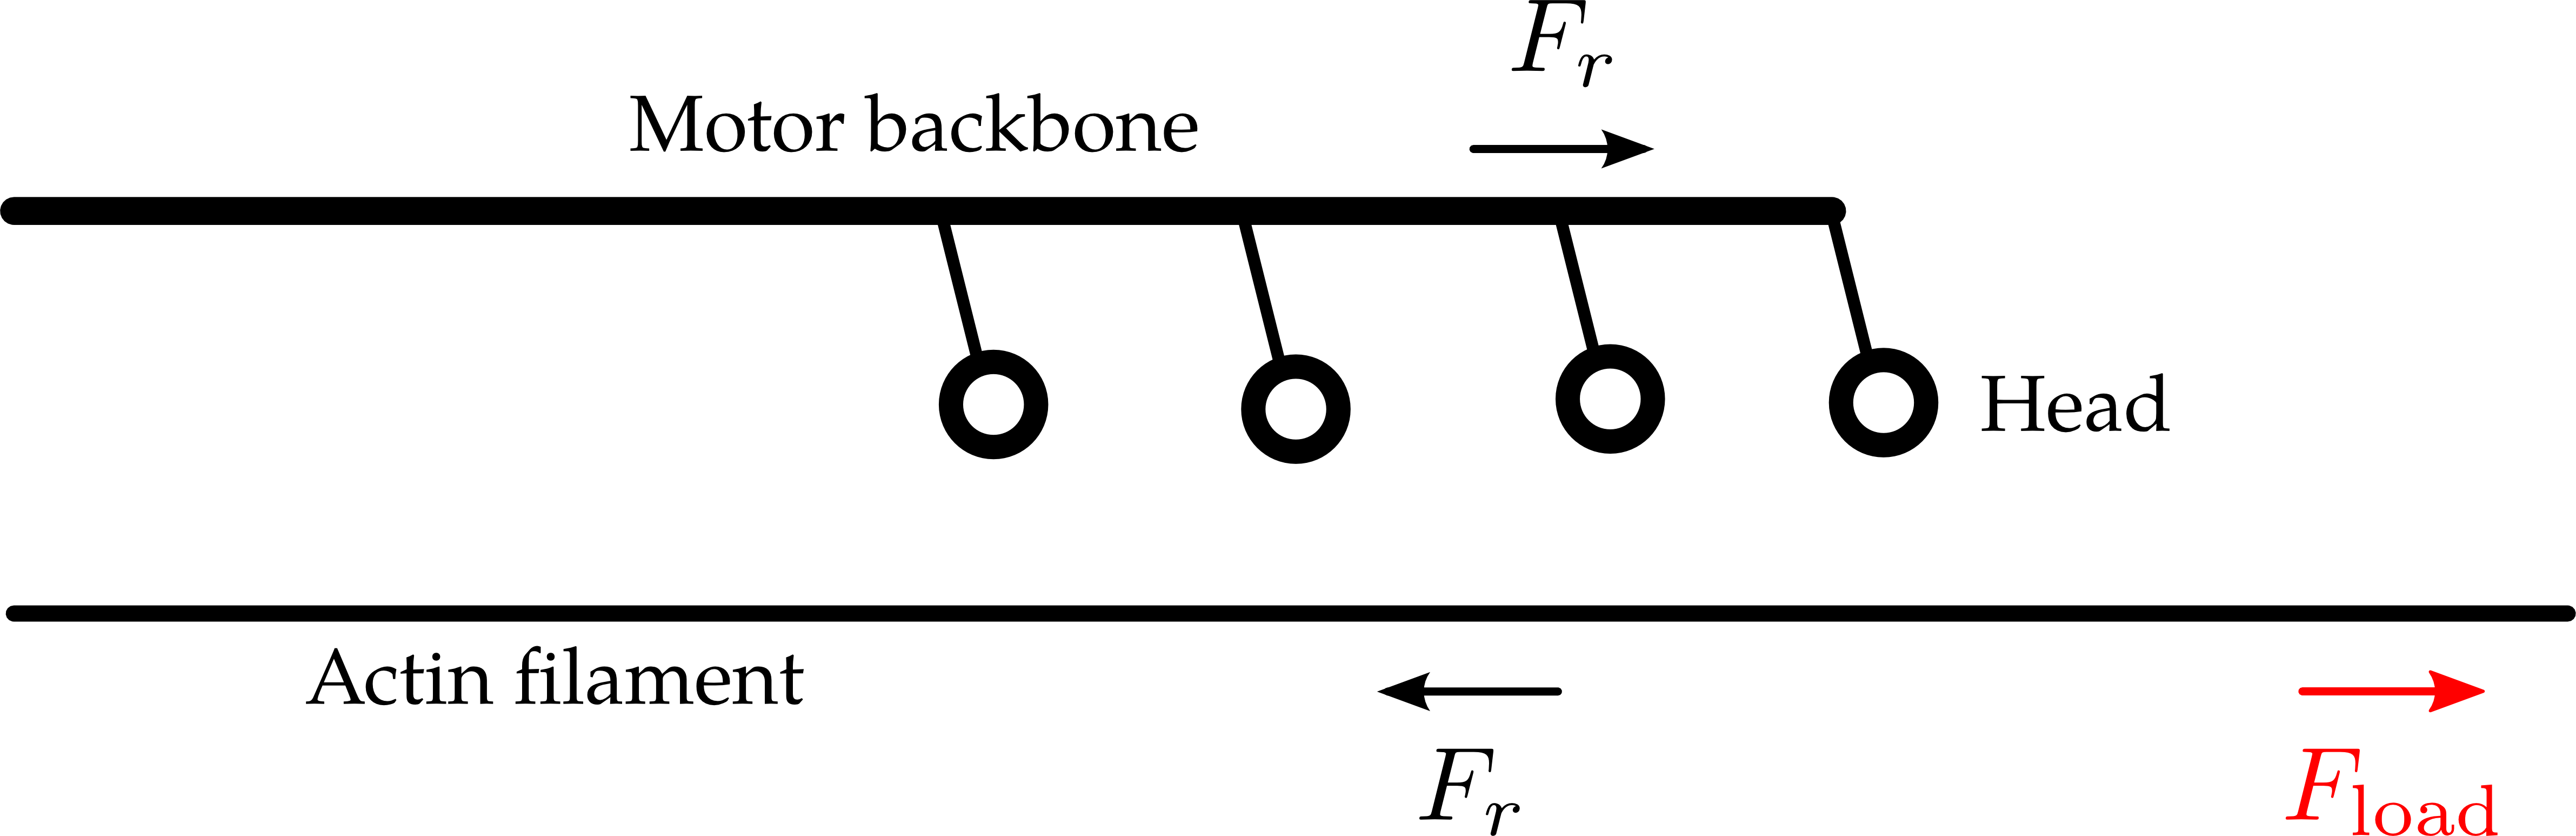
\includegraphics[width=0.45\textwidth,height=!]{load_on_polymer_illustration}
\caption{
\label{fig:load_on_polymer setup}
In this illustration, a variation of the basic setup is shown.  
Now, the load $F_\text{load}$ is applied on actin polymer instead of the myosin motor. Also the orientation of the ratchet along the polymer is reversed.
} 
\end{figure}

As was advertised, the equations of motion are very similar to those of the ``load on the motor'', i.e. \eqref{eq:eom_M} and \eqref{eq:eom_A}.
\begin{align}
&\begin{multlined}[b][.42\textwidth]
\rmd x_\text{M} = 
- \frac{1}{\gamma_\text{M}} \nabla_\text{M} V_t(x_\text{M}(t) - x_\text{A}(t)) \; \rmd t 
\\ 
+ \sqrt{ \frac{2 k_B T}{\gamma_\text{M}} } \; \rmd W_\text{M} ,
\end{multlined}
\label{eq:eom_M_lp} \\
&\begin{multlined}[b][.42\textwidth]
\rmd x_\text{A} = 
\frac{1}{\gamma_\text{A}} \left[ F_\text{load} - \nabla_\text{A} V_t(x_\text{M}(t) - x_\text{A}(t)) \right] \; \rmd t 
\\
+ \sqrt{ \frac{2 k_B T}{\gamma_\text{A}} } \; \rmd W_\text{A} .
\end{multlined}
\label{eq:eom_A_lp}
\end{align}
Note that the argument of the ratchet potential is kept the same, 
while the load $F_\text{load}$ is applied on the polymer and its direction is reversed with respect to the ``load on the motor'' setup. 
This ensures that the mean relative velocity of the motor with respect to the polymer are directly comparable in both setups. 
Another consequence is that the equations of motion of this particular setup can easily be mapped into the ``load on the motor'' setup by interchanging the label of myosin and actin 
along with inverting the x-axis, 
i.e. $\gamma_\text{M}\leftrightarrow\gamma_\text{A}$ and $x_\text{M}\leftrightarrow - x_\text{A}$.


\subsubsection{Tug of war}
\label{sec:tug_of_war}
Another setup, which we investigate, is a natural extension of the previous setup, but now the myosin motor is interacting with two, rather then one, 
anti-parallel actin filaments. 
The external load is again applied directly to filaments instead of the motor, as demonstrated in the figure~\ref{fig:tug_F_illustration}. 
\begin{figure}[t]
\centering
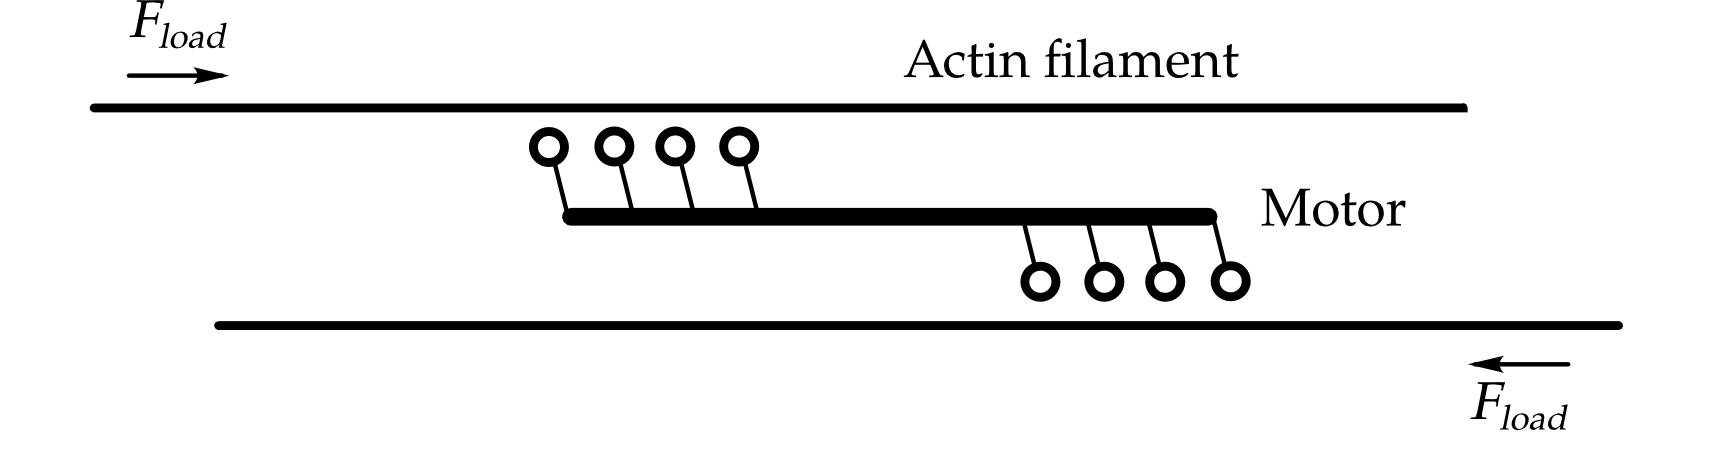
\includegraphics[width=0.45\textwidth,height=!]{tug_F_illustration}
\caption{
\label{fig:tug_F_illustration}
Setup of a motor interacting with two actin filaments that experience equal but opposite loads.
}
\end{figure}
This correspond to a situation when the motor is actively cross-linking two polymers, which are subjected to the tension caused by other motors and other external influences.  

In another words we now have two filaments, denoted by subscript ${\text{A}_1}$ and ${\text{A}_2}$ respectively,
subjected to free diffusion and external load $F_\text{load}$,
which are interacting with the myosin~II motor via the ratchet potential~\eqref{eq:ratchet_interaction}.
This lead to equations of motion 
\begin{equation}
\begin{gathered}
\begin{multlined}[b][.45\textwidth]
\rmd x_\text{M} = 
- \frac{1}{\gamma_\text{M}} \nabla_\text{M} \bigl[ 
V_t(x_{\text{A}_1}(t) - x_\text{M}(t)) 
\\
+ V_t(x_\text{M}(t) - x_{\text{A}_2}(t)) 
\bigr] \; \rmd t 
+ \sqrt{ \frac{2 k_B T}{\gamma_\text{M}} } \; \rmd W_\text{M} ,
\end{multlined}\\
\begin{multlined}[b][.45\textwidth]
\rmd x_{\text{A}_1} = 
- \frac{1}{\gamma_\text{A}} \left[ F_\text{load} + \nabla_{\text{A}_1} V_t(x_{\text{A}_1}(t) - x_\text{M}(t)) \right] \; \rmd t 
\\
+ \sqrt{ \frac{2 k_B T}{\gamma_\text{A}} } \; \rmd W_{\text{A}_1} ,
\end{multlined}\\
\begin{multlined}[b][.45\textwidth]
\rmd x_{\text{A}_2} = 
\frac{1}{\gamma_\text{A}} \left[ F_\text{load} - \nabla_{\text{A}_2} V_t(x_\text{M}(t) - x_{\text{A}_2}(t)) \right] \; \rmd t 
\\
+ \sqrt{ \frac{2 k_B T}{\gamma_\text{A}} } \; \rmd W_{\text{A}_2} ,
\end{multlined}
\end{gathered}
\label{eq:eom_two_actins}
\end{equation}
where the anti-alignment of polymers in substitution of $-x$ instead of $x$ for the second polymer in the argument of the ratchet potential~\eqref{eq:ratchet_interaction}.
Note, that the actin from the ``load on the polymer'' setup correspond to a polymer denoted by $\text{A}_2$ in this setup. 


\subsubsection{Elastic environment}
\label{sec:environment}
As polymers inside the cytoskeleton are usually thoroughly interconnected rather then freely diffusing \cite{blanchoin2014actin,ennomani2016architecture},
we can opt for an alternative approach.
Rather then applying an external load we attach filaments to fixed points by a spring with a constant $k_\text{sp}$, 
similarly to the approach discussed in \cite{albert2014stochastic}. 
These points represent points of interaction with the rest of the network while the spring constant $k_\text{sp}$ represents the elastic properties of the full network. 
The myosin motor is again interacting with two filaments that are arranged in an anti-parallel fashion. 
Hence, similar to the previous case, it will no longer have a preferred direction to move in and 
it eventually reach a steady state where its mean velocity will be zero. 
The observable of interest is now the mean force that the motor applies to the filaments, 
which is measured through the extension of the springs attached to the filaments,
and which represent the active tension in the network produced by the single myosin molecule. 
This setup is sketched in figure \ref{fig:tug}. 
\begin{figure}[t]
\centering
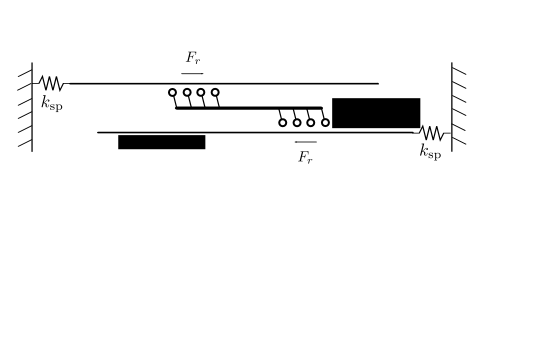
\includegraphics[width=0.45\textwidth,height=!]{tug}
\caption{
\label{fig:tug}
Illustration of a motor pulling on two actin filament that are each connect to a wall by a spring.
}
\end{figure}

The equations of motion are then just a modification of \eqref{eq:eom_two_actins}  
\begin{equation}
\begin{gathered}
\begin{multlined}[b][.45\textwidth]
\rmd x_\text{M} = 
- \frac{1}{\gamma_\text{M}} \nabla_\text{M} \bigl[ 
V_t(x_{\text{A}_1}(t) - x_\text{M}(t)) 
\\
+ V_t(x_\text{M}(t) - x_{\text{A}_2}(t)) 
\bigr] \; \rmd t 
+ \sqrt{ \frac{2 k_B T}{\gamma_\text{M}} } \; \rmd W_\text{M} ,
\end{multlined}\\
\begin{multlined}[b][.45\textwidth]
\rmd x_{\text{A}_1} = 
- \frac{1}{\gamma_\text{A}} \bigl[ \nabla_{\text{A}_1} V_t( x_{\text{A}_1}(t) - x_\text{M}(t) ) 
\\
+ k_\text{sp} \left( x_{\text{A}_1}(t) - x_{\text{A}_1}(0) \right) \bigr] \; \rmd t 
+ \sqrt{ \frac{2 k_B T}{\gamma_\text{A}} } \; \rmd W_{\text{A}_1} ,
\end{multlined}\\
\begin{multlined}[b][.45\textwidth]
\rmd x_{\text{A}_2} = 
- \frac{1}{\gamma_\text{A}} \bigl[ \nabla_{\text{A}_2} V_t( x_\text{M}(t) - x_{\text{A}_2}(t) )
\\
+ k_\text{sp} \left( x_{\text{A}_2}(t) - x_{\text{A}_2}(0) \right) \bigr] \; \rmd t 
+ \sqrt{ \frac{2 k_B T}{\gamma_\text{A}} } \; \rmd W_{\text{A}_2} ,
\end{multlined}
\end{gathered}
\label{eq:eom_two_actins_no_load}
\end{equation}
where the load is replaced by the force caused by springs and where the reference point for the springs is chosen as their position at the initial time. 

\subsection{Numerical method}
We use an Euler-Maruyama integration scheme to stochastically evolve the systems from a randomized initial configuration \cite{kloeden1989survey,maruyama1955continuous}. 
Most results are obtained after evolving the system up to a time of $1\;\mathrm{s}$ with time step $\Delta t = 0.01\;\mathrm{ns}$ and averaging over $100$ independent copies.    
An exception is the data in figure \ref{fig:tug_k}, 
which was obtained after an ergodic average every $1\;\mathrm{ms}$ over $10\;\mathrm{s}$ with time step $\Delta t = 0.01\;\mathrm{ns}$ and ensemble average over $1000$ independent copies.
Lastly, to obtain the empirical distribution in figure \ref{fig:pos_distr}, 
data was gathered by sampling every $0.5\;\mathrm{ms}$ for a total time of $1\;\mathrm{s}$ with time step $\Delta t = 0.001\;\mathrm{ns}$ and from $100$ independent simulations and converted into a histogram with a bin width of $0.1\;\mathrm{nm}$.


\section{Mean velocity}
\label{sec:velocity}
At first, we study the mean velocity of the motor with four heads with respect to the filament in the ``load on the motor'' setup,
\begin{equation}
\langle v \rangle 
= \frac{ \left\langle \rmd x_\text{M} \right\rangle }{ \rmd t } 
- \frac{ \left\langle \rmd x_\text{A} \right\rangle }{ \rmd t } ,
\label{eq:mean_velocity} 
\end{equation}
for different values of the scaling factor $c$ and without any external load $F_\text{load} = 0$.
Note that in this particular case, where there is no external load, setups ``load on the motor'' and ``load on the polymer'' coincide. 

The results are shown in the figure~\ref{fig:c_v},
\begin{figure}[t]
\centering
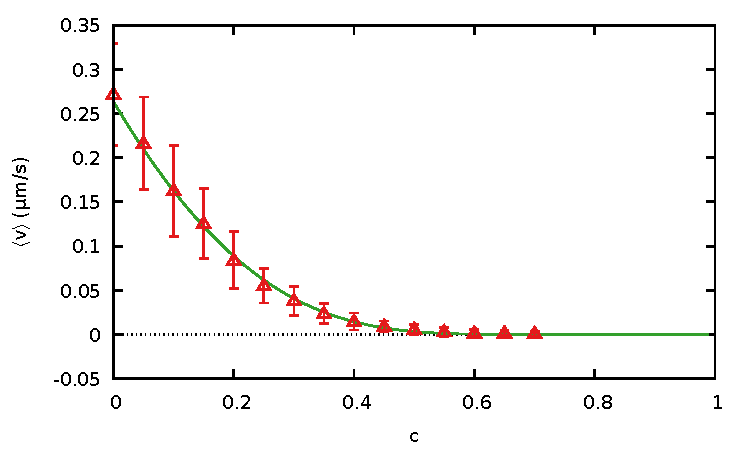
\includegraphics[width=0.45\textwidth,height=!]{c_v_4heads}
\caption{
\label{fig:c_v}
Mean velocity $\langle v \rangle$ of the motor relative to the actin filament for $c \in (0,1)$.
The mean velocity rapidly decreases towards the $0$ as we approach equilibrium, $c \to 1$.  
Green line correspond to the fit $ \left\langle v \right\rangle \propto \exp ( - \frac{\alpha}{1-c} ) $.
%The dependency is guessed, unfortunately I don't have any argument to support it. 
} 
\end{figure}
where we see that the mean velocity has a maximum at $c=0$ and goes to zero when $c$ approaches $1$. 
This is to be expected since $c=1$ corresponds to equilibrium, where there is no difference between the two internal states, cf.~\eqref{eq:transition}.
On the other hand, for $c=0$ we have the biggest discrepancy between the two internal states of each head. 


Secondly, the mean velocity~\eqref{eq:mean_velocity} also depends on the concentration of ATP through the binding rate $k_\text{bind}$. 
In this setup, we fix the ATP unbinding rate $k_\text{unbind}$ and scaling factor $c$, cf. table~\ref{tab:parameters}, and vary the ATP binding rate $k_\text{bind}$. 
The resulting dependency is shown in the figure~\ref{fig:v_k}. 
\begin{figure}[t]
\centering
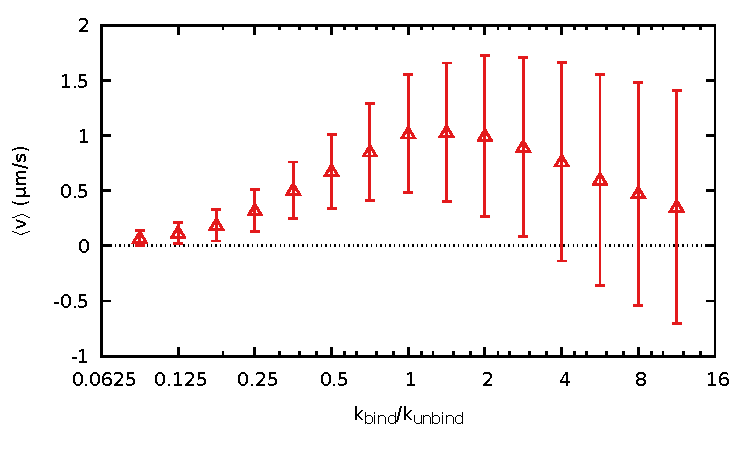
\includegraphics[width=0.45\textwidth,height=!]{v_k}
\caption{
\label{fig:v_k} 
Mean velocity of the motor relative to the actin filament $\langle v \rangle$ for varying $k_\text{bind}$.
The velocity decreases to $0$ for large discrepancies between binding and unbinding rate and reaches maximum when they are comparable.
}
\end{figure}
We observe that the maximal velocity is reached for rates close to $k_\text{bind} = k_\text{unbound}$. 
Departing far from this ratio means that one of the states become dominant and thus the system effectively approaches equilibrium.  
The main difference between the $k_\text{bind}/k_\text{unbind}$ being low or high is the amplitude of the interaction with actin. 
In the ATP bound state the interaction is weaker, 
which is reflected in the fact that the system is trapped for shorter times close to the local minimums and diffuses more. 
Hence, the variance of the relative velocity is higher when compared to the ATP unbound state. 


\section{Force -- velocity relation}
\label{sec:force-velocity}
In the previous section, we have investigated the mean relative velocity for motor in the ``load on the motor'' setup without any external load. 
Here we will focus on the dependency of the mean relative velocity \eqref{eq:mean_velocity} on an external load force $F_\text{load}$ applied on the motor anti-parallel to the preferred direction, 
cf. figure~\ref{fig:ratchet_setup}.

Figure~\ref{fig:F_v} shows the typical force -- mean velocity relations for various ATP binding rates $k_\text{unbind}$, which mimics the dependency on ATP concentration.
\begin{figure}[t]
\centering
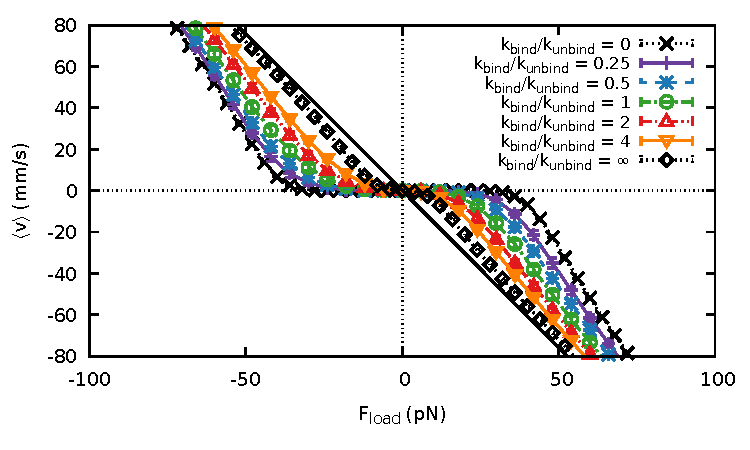
\includegraphics[width=0.45\textwidth,height=!]{F_v}
\caption{
\label{fig:F_v} 
Mean velocity $\langle v \rangle$ of the motor as a function of the load force $F_\text{load}$ for $c=0.3$ and for various ATP binding rate $k_\text{bind}$.
Solid black line correspond to a situation where there will be no interaction with the actin filament, i.e. $\langle v \rangle = - F_\text{load} / \gamma_\text{M}$. 
}
\end{figure}
For small load forces, the interaction with an actin polymer provides an additional friction force countering the load force, 
which results in small response of the relative velocity $\langle v \rangle$.
For larger forces the system looses its resilience and the contribution from the load will dominate. 
The larger the load, the more the velocity will approach the velocity of a non-interacting motor, $\langle v \rangle = - \frac{1}{\gamma_\text{M}} F_\text{load}$.
This will be exactly proven later on, in section \ref{sec:ind_velo}. 
Curves for higher ATP binding rates are closer to the curve for the completely unbound motor.
As the motor is more loosely bound to the polymer, it is more submissive to the external load.
Such a force-velocity relation was already presented in 2002 by Reimann \cite{reimann2002brownian} for a flashing ratchet, representing a motor with a single head.

A similar plot is shown in figure \ref{fig:F_v_heads}, where instead of varying ATP binding rate $k_\text{bind}$ we look at motors with different numbers of heads $N$. 
\begin{figure}[t]
\centering
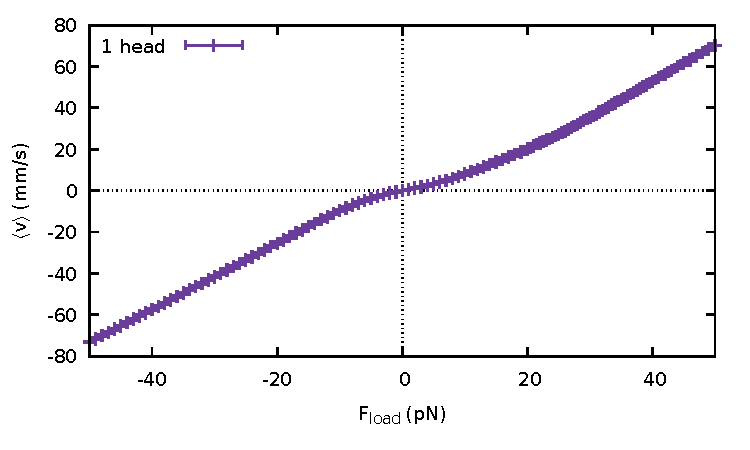
\includegraphics[width=0.45\textwidth,height=!]{F_v_heads}
\caption{
\label{fig:F_v_heads} 
Mean velocity $\langle v \rangle$ of the motor as a function of the load force $F_\text{load}$ for $c=0.3$ and for motors with different number of heads $N$.
Solid black line correspond to a non-interacting motor, i.e. $\langle v \rangle = - F_\text{load} / \gamma_\text{M}$. 
}
\end{figure}
Motors with only one head are very susceptible to external loads and the force from the ratchet offers little resistance. 
On the other hand, the motors with four and sixteen heads have almost identical force-velocity relations. 
However, it would be na\"{\i}ve to consider these motors identical as they behave very differently regarding their energetics,  
which we will discuss in the section~\ref{sec:efficiency}.

In figure~\ref{fig:F_v_setups} we compare the force-velocity relation of the ``load on the motor'' setup with alternative setups,
namely with the ``load on the polymer'', cf. section~\ref{sec:load_on_polymer} and the ``tug of war'', cf. section~\ref{sec:tug_of_war}.
\begin{figure}[t]
\centering
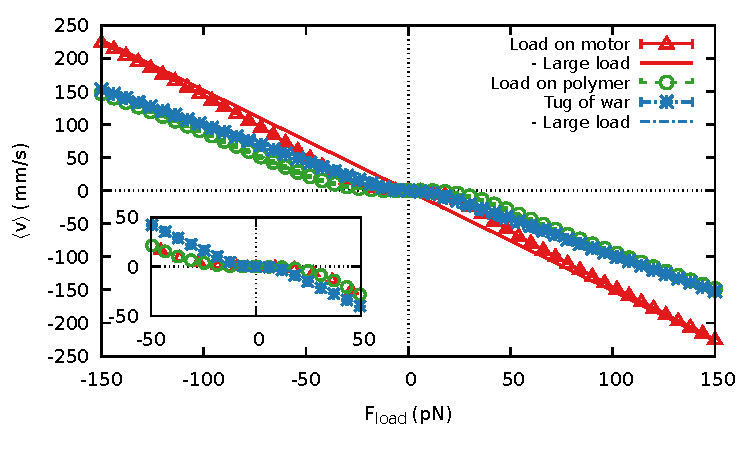
\includegraphics[width=0.45\textwidth,height=!]{F_v_setups}
\caption{
\label{fig:F_v_setups} 
Mean velocity $\langle v \rangle$ of the motor with respect to the filament, as a function of the load force $F_\text{load}$ for different various setups.
For large loads, the curves approach either  $ - F_\text{load} / \gamma_\text{M}$ or $ - F_\text{load} / \gamma_\text{A}$, depending on whether the load is applied to the motor or to the polymer. 
Inset: Force-velocity plotted with rescaled x-axes,
$F_\text{load} \to - F_\text{load} / \gamma_\text{M}$ for the ``load on the motor'' setup 
and $F_\text{load} \to - F_\text{load} / \gamma_\text{A}$ for the ``load on the filament'' and the ``tug of war'' setup. 
}
\end{figure}
Note that for the ``tug of war'' setup we have two equivalent choices for the relative velocity,
however due to the symmetry of the setup, cf. figure~\ref{fig:tug_F_illustration}, in the steady state these options differ only by sign, 
hence we define the relative velocity~\eqref{eq:mean_velocity} as 
\[
\langle v \rangle 
\equiv \frac{ \left\langle \rmd x_\text{M} \right\rangle }{ \rmd t }
- \frac{ \left\langle \rmd x_{\text{A}_2} \right\rangle }{ \rmd t }
= - \left( \frac{ \left\langle \rmd x_\text{M} \right\rangle }{ \rmd t }
- \frac{ \left\langle \rmd x_{\text{A}_1} \right\rangle }{ \rmd t } \right) .
\]
For small loads, the mean relative velocity $\langle v \rangle$ of the motor with respect to the polymer remains close to each other in all setups.
However, for high loads a clear difference in their asymptotic behavior becomes apparent.
When the load is applied to the motor the relative velocity goes to $ - F_\text{load} / \gamma_\text{M}$.
For the setups where the load is applied to the filaments, the relative velocity goes to $ - F_\text{load} / \gamma_\text{A}$ with increasing load.

In the inset of figure~\ref{fig:F_v_setups}, 
the force-velocity relations are plotted on rescaled x-axes for the different setups, 
which takes the difference in their asymptotic behavior into account. 
Thus, the ``load on the motor'' setup is plotted with respect to $ - F_\text{load} / \gamma_\text{M}$ instead of $F_\text{load}$,
while the other setups are plotted with respect to $ - F_\text{load} / \gamma_\text{A}$.
The curve for the simplest setups, with one motor and one polymer, collapse in this plot, 
confirming the fact that they can be mapped onto each other by switching friction coefficients $\gamma_\text{M} \leftrightarrow \gamma_\text{A}$ 
and reversing the relative velocity. 
However, the ``tug of war'' setup manifests a clear difference for mid-range loads due to the more complex interaction with two polymer. 

\subsection{Stall force}
From figure~\ref{fig:F_v} it is apparent that when applying a force against the preferred direction of the motor, 
the motor first slows down until it stops before it reverses its direction. 
The force magnitude that is needed to stop the motor's movement relative to the actin filament is called the stall force $F_\text{stall}$,  
\[
\left\langle v ( F_\text{load} \equiv F_\text{stall} ) \right\rangle = 0 .
\]
Figure~\ref{fig:F_v_zoom} shows a zoomed in version of figure~\ref{fig:F_v} for small loads, opposite to the motor's preferred direction of motion. 
\begin{figure}[t]
\centering
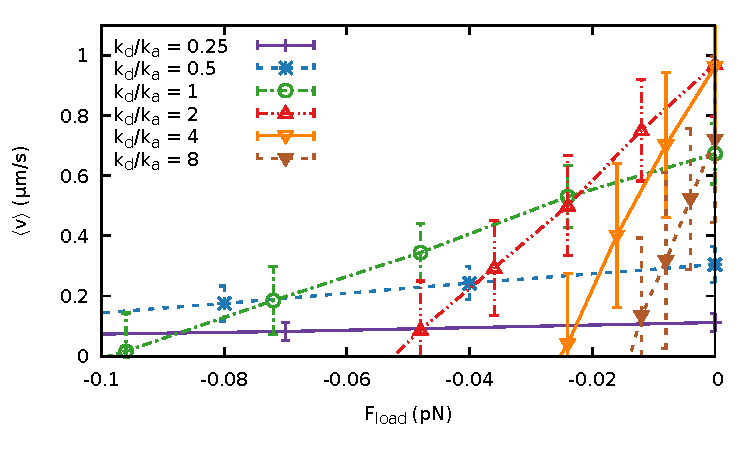
\includegraphics[width=0.45\textwidth,height=!]{F_v_zoom}
\caption{
\label{fig:F_v_zoom} 
Mean velocity of the motor $\langle v \rangle$ with a small load force $F_\text{load}$ applied in the direction opposing the movement for different ATP binding rates $k_\text{bind}$.
Intersections with the $x$ axis correspond to stall forces $F_\text{stall}$ for given detach rates. 
We can see that with increasing $k_\text{bind}/k_\text{unbind}$ ratio the slope increases as well as the full curve shifts in the low force region, causing a persistent decrease in stall force. 
}
\end{figure}
The intersections with the horizontal axis correspond to stall forces,  
while intersections of the curves with the vertical axis correspond to the mean velocities for system without any external load, compare figure~\ref{fig:v_k}. 
We see that for small loads the mean velocity decreases linearly with increasing load. 
Moreover, the slope of the force -- mean velocity relation increases with the binding rate $k_\text{bind}$. 
This is responsible for monotonous decrease of the stall force $F_\text{stall}$ with respect to the ATP binding rate $k_\text{bind}$, see figure~\ref{fig:k_Fstall}.
\begin{figure}[t]
\centering
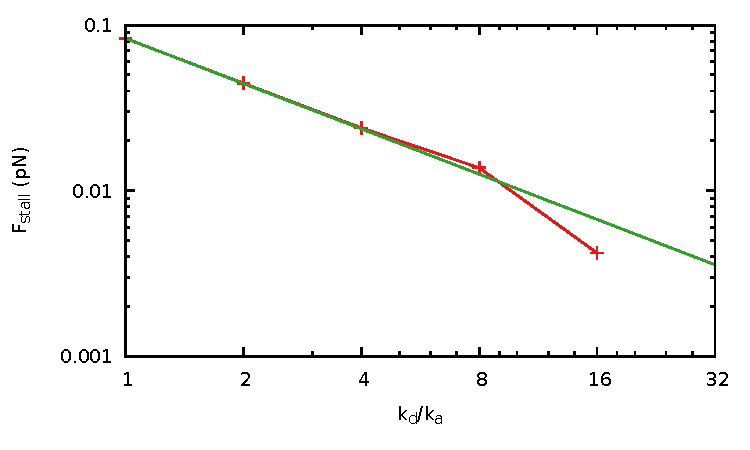
\includegraphics[width=0.45\textwidth,height=!]{k_Fstall}
\caption{
\label{fig:k_Fstall} 
Stall force $F_\text{stall}$ for different detach rates $k_\text{d}$.
We observe power-law decay $F_\text{stall} \propto k_\text{d}^{-\alpha}$ with exponent $\alpha = 1.002 \pm 0.014$. 
}
\end{figure}
When the ATP binding rate increases, so does the fraction of time in which the motor is weakly interacting with the actin filament. 
Hence, on average it will take a smaller load to halt a motor since the amplitude of its confining potential will be typically lower.
Ultimately, when the system is found only in the ATP unbound state the relative mean velocity is zero, $\langle v \rangle = 0$, as the system reached an equilibrium 
and thus the stall force reaches zero as well, $F_\text{stall} \to 0$.
%TODO Relate to power law => Maybe some analytics can help

\subsection{Velocity with respect to medium}
\label{sec:ind_velo}
Until now, we have investigated the relative velocity of the myosin and actin polymer \eqref{eq:mean_velocity}, however this does not give us additional information of
whether it is the motor that is moving with respect to the medium or rather the actin polymer that is being pushed back through the medium.
In order to find the dependency between individual velocities and relative velocity in the ``load on the motor'' setup, 
we start by taking expectation values of their equations of motion, cf. equations~\eqref{eq:eom_M} and~\eqref{eq:eom_A},
\begin{align}
\gamma_\text{M} \langle v_\text{M} \rangle &= \frac{ \langle \rmd x_\text{M} \rangle }{\rmd t} = \langle F_\text{r} \rangle - F_\text{load} , 
\label{eq:pre_velocity_M} 
\\
\gamma_\text{A} \langle v_\text{A} \rangle &= \frac{ \langle \rmd x_\text{A} \rangle }{\rmd t} = -\langle F_\text{r} \rangle , 
\label{eq:pre_velocity_A}
\end{align}
where $F_\text{r}$ denote ratchet force, 
\begin{equation}
F_\text{r} = - \nabla_\text{M} V_t( x_\text{M} - x_\text{A} ) = \nabla_\text{A} V_t(x_\text{M} - x_\text{A} ) . 
\label{eq:ratchet_force}
\end{equation}
Next, we express the relative velocity \eqref{eq:mean_velocity} in terms of the mean ratchet force $\langle F_\text{r} \rangle$ and the external load $F_\text{load}$  
\begin{equation}
\langle v \rangle 
= \langle v_\text{M} - v_\text{A} \rangle 
= \frac{\gamma_\text{A} + \gamma_\text{M}}{\gamma_\text{A} \gamma_\text{M}} \langle F_\text{r} \rangle - \frac{1}{\gamma_\text{M}} F_\text{load} ,
\label{eq:mean_velocity_Fr_Fl}
\end{equation}
which leads to individual velocities expressed in terms of the mean velocity and load 
\begin{align}
\langle v_\text{M} \rangle &= \frac{1}{ \gamma_\text{A} + \gamma_\text{M} } \left( \gamma_\text{A} \langle v \rangle - F_\text{load} \right) ,
\label{eq:velocity_M} \\
\langle v_\text{A} \rangle &= -\frac{1}{ \gamma_\text{A} + \gamma_\text{M} } \left( \gamma_\text{M} \langle v \rangle + F_\text{load} \right) .
\label{eq:velocity_A}
\end{align}

Note, that for the load equal the stall force, $F_\text{load} = F_\text{stall}$, both velocities are equal and non-zero.
This is related to the fact that the full system is moving with respect to the liquid, as can be seen from the mean velocity of the geometric center 
\begin{multline*}
\langle v_\text{center} \rangle = \left\langle \frac{ v_\text{M} + v_\text{A} }{2} \right\rangle 
= \\
= \frac{ \gamma_\text{A} - \gamma_\text{M} }{ 2 ( \gamma_\text{A} + \gamma_\text{M} ) } \langle v \rangle - \frac{1}{ \gamma_\text{A} + \gamma_\text{M} } F_\text{load}
, 
\end{multline*}
which is proportional to both the load and the relative velocity and is zero only when $\langle v \rangle = 2 F_\text{load} / ( \gamma_\text{A} - \gamma_\text{M} )$.

Also note, that the ratchet force is bounded by 
\[
- \frac{ N V }{ \ell (1-a) } 
\le 
F_\text{r}
\le
\frac{ N V }{ \ell a } ,
\]
cf. equations~\eqref{eq:ratchet_potential} and~\eqref{eq:ratchet_interaction}, 
which means that there is a maximal portion of the load that the ratchet interaction can transmit from the motor to the polymer 
and thus there exists an upper and lower bound for the polymer's velocity~\eqref{eq:pre_velocity_A}.   
This can be seen in the figure~\ref{fig:ind_v} depicting the individual velocities as a function of the external load $F_\text{load}$,  
\begin{figure}[t]
\centering
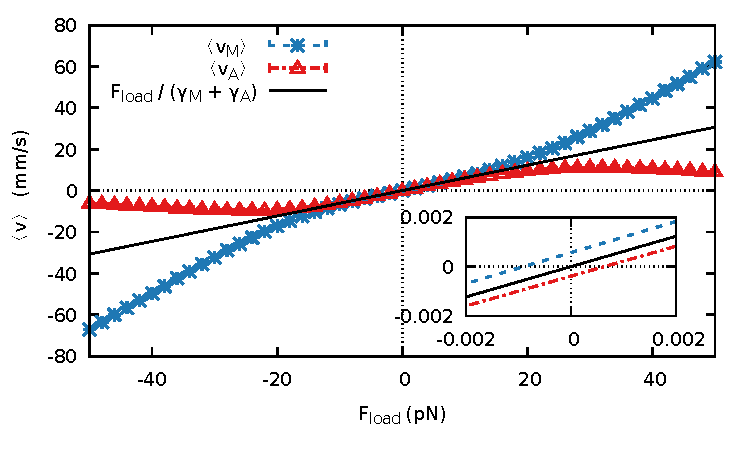
\includegraphics[width=0.45\textwidth,height=!]{individual_velocities}
\caption{
\label{fig:ind_v} 
Mean velocities of the motor and actin filament with respect to an inertial frame of reference for $k_\text{bind}/k_\text{unbind} = 2$.
We observe that only the myosin is moving while the velocity of the dragged actin filament decreases as we increase the load on the myosin motor.
Inset: Zoomed to the linear regime around the origin.
}
\end{figure}
where the polymer's velocity is clearly bounded. 

For small loads, the motor and actin filament are moving together, as the coupling by the ratchet interaction proves to be dominant. 
This hypothesis can be further supported by the linear dependency of equations~\eqref{eq:velocity_M} and~\eqref{eq:velocity_A} on the load, 
which is due to the fact that for small loads also the mean relative velocity \eqref{eq:mean_velocity} is linear in the load, see figure~\ref{fig:F_v}. 
Moreover as the mean velocity's response to the external force is typically very small compared to the direct contribution from the external load to the individual velocities,
we can be further approximate them by  
\begin{align*}
\left\langle v_\text{M} \right\rangle 
&\approx - \frac{ F_\text{load} }{ \gamma_\text{A} + \gamma_\text{M} } + \frac{ \gamma_\text{A} }{ \gamma_\text{A} + \gamma_\text{M} } \left\langle v \right\rangle_{ F_\text{load} = 0 },
\\
\left\langle v_\text{A} \right\rangle 
&\approx - \frac{ F_\text{load} }{ \gamma_\text{A} + \gamma_\text{M} } - \frac{ \gamma_\text{M} }{ \gamma_\text{A} + \gamma_\text{M} } \left\langle v \right\rangle_{ F_\text{load} = 0 } .
\end{align*}
Such a response is depicted in the inset of the figure~\ref{fig:ind_v}, where the shift in individual velocities caused by the relative velocity for very small loads is constant.

Since the load is only applied to the motor in this setup, for very high loads, the motor will start slipping over the ratchet potential along the actin filament. 
Consequently, the actin filament's mean velocity will stop increasing and eventually approaches zero, 
while the myosin motor's mean velocity goes to $\langle v_\text{M} \rangle \asymp F_\text{load}/\gamma_\text{M} $
as can be seen in figure~\ref{fig:ind_v}. 
This is due to the fact that the asymptotic behavior of the relative velocity  is
\[
\langle v \rangle \asymp - \frac{ F_\text{load} }{\gamma_\text{M} },
\]
which can be obtained directly from equation~\eqref{eq:mean_velocity_Fr_Fl} as the contribution from the ratchet force is bounded.
The asymptotic behavior for the motor and the polymer follows from equations~\eqref{eq:velocity_M} and~\eqref{eq:velocity_A} for $ \left\langle v \right\rangle = - F_\text{load} / \gamma_\text{M} $. 
From there it is also apparent that the relative mean velocity in the limit of infinitely large load $F_\text{load} \to \pm \infty$ will be equal to the motor's velocity $\langle v_\text{M} \rangle$.
This is agrees with the data in figure~\ref{fig:F_v}.

\subsection{Ratchet force} 
One can interpret the nonlinear force-velocity relation for the myosin~\eqref{eq:pre_velocity_M} as balance between the load, drag force and the force caused by the ratchet interaction, 
that intrinsically depends on the load. 
Without the ratchet interaction, the motion of the myosin would satisfy $ \gamma_\text{M}\langle v\rangle = -F_\text{load}$. 
The discrepancy in this relation, up to a pre-factor, equals the mean force exerted via the flashing ratchet $\langle F_\text{r}\rangle$, 
cf. equation~\eqref{eq:mean_velocity_Fr_Fl},
\begin{equation}
\frac{\gamma_\text{A}\gamma_\text{M}}{\gamma_\text{A} + \gamma_\text{M} } \left(\langle v \rangle + \frac{F_\text{load}}{\gamma_\text{M}}\right) = \langle F_\text{r} \rangle.
\label{eq:mean_ratchet_force}
\end{equation}
Note that this is the same as the distance between the force-velocity curves and the ratchet-free curve in figure~\ref{fig:F_v}. 
Also note that, using the re-scaled parameters \eqref{eq:rescale_parameters} introduce in the appendix, 
we can write the mean ratchet force as $\langle F_\text{r} \rangle = \gamma^* \langle v \rangle - F^*$.
In figure~\ref{fig:ratchet_force} we show, 
that the response of the system for small loads is linear and independent of the chemical rates and hence of the ATP concentration. 
\begin{figure}[t]
\centering
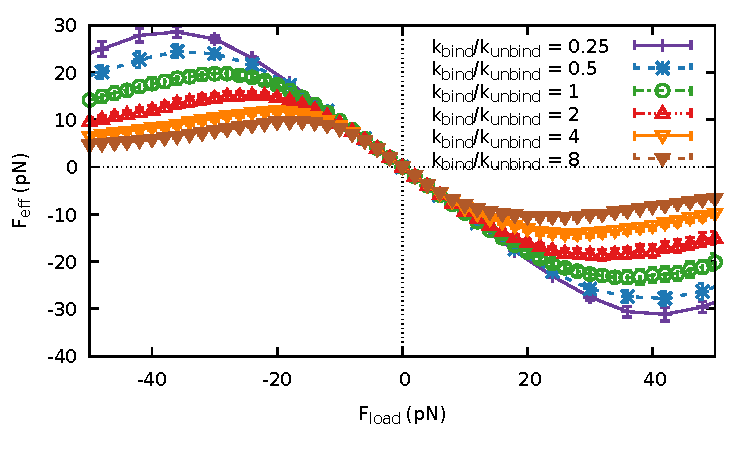
\includegraphics[width=0.45\textwidth,height=!]{ratchet_force}
\caption{
\label{fig:ratchet_force}
Mean force from the ratchet interaction depending on the load force on the motor for several values of $k_\text{bind}$. 
For small loads, the ratchet force completely counter to load, hence the linear regime around $F_\text{load}=0$ goes like
}
\end{figure}
In this regime the motor hardly moves along the filament and the load is almost completely countered by the mean ratchet force, i.e. it acts as a friction force.
With increasing load, the force generated by the ratchet interaction will reach a maximal value and eventually decay for larger external load forces. 
In the appendix, cf. equation~\eqref{eq:mean_velocity_large}, we show that the friction provided by the ratchet will go to zero as the load goes to infinity as 
\begin{equation}
\left| \langle F_\text{r} \rangle_{F_\text{load}\rightarrow\infty} \right| \asymp \frac{1}{F_\text{load}} , 
\label{eq:ratchet_vs_load}
\end{equation} 
which is depicted in figure~\ref{fig:ratchet_force_decay}. 
\begin{figure}[t]
\centering
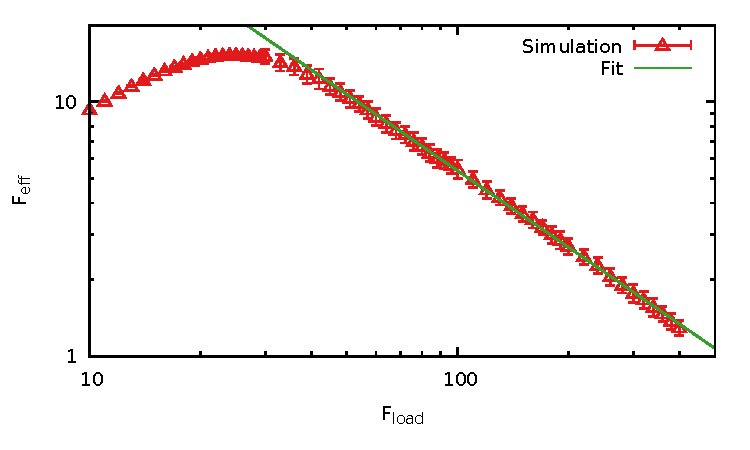
\includegraphics[width=0.45\textwidth,height=!]{ratchet_force_decay}
\caption{
\label{fig:ratchet_force_decay}
The ratchet force, depending on the load, is shown in a logarithmic plot. 
We can see that the ratchet force asymptotically decays according to the power law $F_\text{eff} \propto F_\text{load}^{-\alpha}$, 
with exponent determined from the fit to be $\alpha = 0.9990 \pm 0.0047$, 
which is in good agreement with the theoretical prediction~\eqref{eq:ratchet_vs_load}.
}
\end{figure}


\subsection{Tension in the motor}
The force-velocity relation can also be exploited to obtain the tension in the motor. 
Since both the load and ratchet force are directly applied on the respective ends of the motor, 
the tension applied to the motor $\tau_\text{M}$ is proportional to their difference,
where we choose the sign of the tension in such a way 
that the positive value corresponds to a pair of forces applied on each end of the motor in the direction away from the motor,
i.e.  
\begin{align}
\left\langle \tau_\text{M} \right\rangle 
&= \langle F_\text{r} \rangle + F_\text{load} \nonumber \\
&= \frac{\gamma_\text{A}\gamma_\text{M}}{\gamma_\text{A}+\gamma_\text{M}}\langle v\rangle 
+ \left(1 + \frac{\gamma_\text{A}}{\gamma_\text{A}+\gamma_\text{M}} \right) F_\text{load}.
\label{eq:tension}
\end{align}
Note, that we omit the normalization by the length of the motor as it is just a division by a constant due to the infinite rigidity of the motor in our model.   
In a similar fashion we can as well define the tension on the polymer as
\begin{align}
\left\langle \tau_\text{A} \right\rangle 
&= - \langle F_\text{r} \rangle \nonumber \\
&= - \frac{\gamma_\text{A}\gamma_\text{M}}{\gamma_\text{A}+\gamma_\text{M}}\langle v\rangle 
- \frac{\gamma_\text{A}}{\gamma_\text{A}+\gamma_\text{M}} F_\text{load}.
\label{eq:tension_on_polymer}
\end{align}

We plot the tension on the motor as a function of the load $F_\text{load}$ in figure~\ref{fig:tension} for various ATP binding rates 
\begin{figure}
\centering
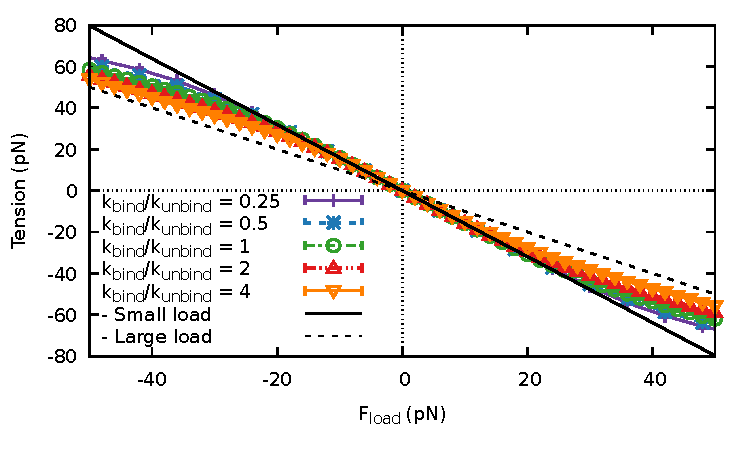
\includegraphics[width=.45\textwidth,height=!]{tension.pdf}
\caption{\label{fig:tension}
The dependency of the tension~\eqref{eq:tension} on the load force $F_\text{load}$ for different ATP binding rates $k_\text{bind}$.
We can see that with increasing ATP binding rate there is a faster departure from the small load regime towards the large load asymptotic behavior. 
}
\end{figure}
and in figure~\ref{fig:tension_heads} as a function of the amount of heads on a motor $N$. 
\begin{figure}
\centering
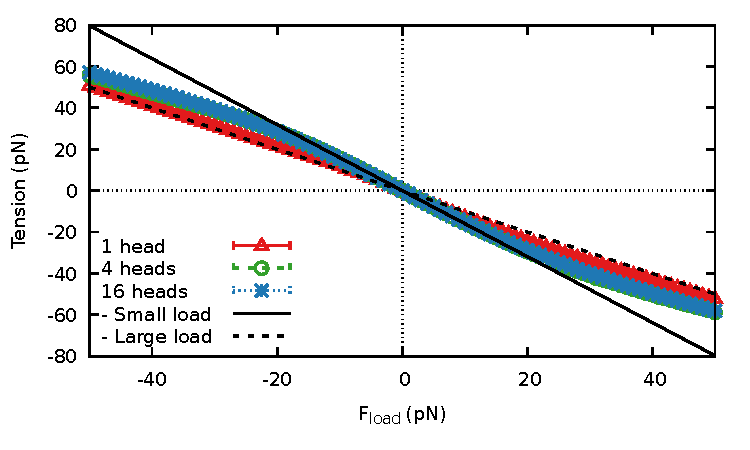
\includegraphics[width=.45\textwidth,height=!]{tension_heads.pdf}
\caption{\label{fig:tension_heads}
The dependency of the tension~\eqref{eq:tension} on the load force $F_\text{load}$ for different number of heads. 
We observe a similar behavior as in figure~\ref{fig:tension} for the motor with four and sixteen heads which seems to be indistinguishable, 
while the motor with a single head departs very rapidly from the low force regime. 
}
\end{figure}
We observe that for small loads the tension is linear in load, this is in good agreement with the observation of the plateau in force velocity relation, 
see figure~\ref{fig:F_v}.
In this regime, the velocity is small compared to the initial load as most of the load is countered by the ratchet interaction, 
hence only the second term in~\eqref{eq:tension} contributes, 
\begin{equation}
\left\langle \tau_\text{M} \right\rangle
\approx
\left(1 + \frac{\gamma_\text{A}}{\gamma_\text{A}+\gamma_\text{M}} \right) F_\text{load}.
\label{eq:tension_low_load} 
\end{equation}

For large force, the motor slips over the potential and thus the mean ratchet force $\langle F_\text{r}$ approaches zero,
as can be seen in figures~\ref{fig:ratchet_force} and~\ref{fig:ratchet_force_decay}.
Hence, the large force asymptotic is given solely by the load
\begin{equation}
\left\langle \tau_\text{M} \right\rangle
\asymp F_\text{load} 
\qquad \text{for} \qquad F_\text{load} \to \pm \infty. 
\label{eq:tension_large_load}
\end{equation}
This is further supported by calculations of the mean velocity for a motor with a single head, provided in the appendix, cf. equation~\eqref{eq:mean_velocity_large}.


\subsubsection{Load on the polymer}
A similar analysis can be made for alternative setups presented in section~\ref{sec:other_setups}. 
In the case where the load is applied directly to the polymer instead of the motor, cf. setup ``load on the polymer'' introduced in the section~\ref{sec:load_on_polymer}, 
the motor only experiences a force from the ratchet interaction with the polymer and not from a load. 
Therefore, the tension on the motor is given only by the mean ratchet force,  
cf. the equation~\eqref{eq:mean_ratchet_force},  
where the load must be divided by $\gamma_\text{A}$ since the load is exerted on the actin filament instead of the motor,
i.e.
\begin{equation}
\left\langle \tau_\text{M} \right\rangle 
= \langle F_\text{r} \rangle 
= \frac{\gamma_\text{A}\gamma_\text{M}}{\gamma_\text{A} + \gamma_\text{M} } \left(\langle v \rangle + \frac{F_\text{load}}{\gamma_\text{A}}\right) . 
\label{eq:tension_load_on_polymer}
\end{equation}
Following the same argumentation as in the ``load on the motor'' setup, for small loads, the tension will be given by
\begin{equation}
\left\langle \tau_\text{M} \right\rangle
\approx \frac{\gamma_\text{M}}{\gamma_\text{A}+\gamma_\text{M}} F_\text{load}.
\label{eq:tension_low_load_on_polymer}
\end{equation}
This is similar to~\eqref{eq:tension_low_load}, where the motor experiences the load directly, up to an exchange of friction coefficients of the motor and actin filament. 

Furthermore, since the load is not directly applied to the motor in this setup, the overall term $F_\text{load}$ is not present. 
Therefore, the tension vanishes for large load in the same way that the relative velocity approaches $-F_\text{load} / \gamma_\text{A}$, see~\eqref{eq:ratchet_vs_load},
\begin{equation}
\langle \tau_\text{M} \rangle 
\propto
F_\text{load}^{-1}
\qquad\text{for}\qquad
F_\text{load} \to \infty 
.
\label{eq:tension_load_on_polymer_large}
\end{equation}


\subsubsection{Tug of war}
In the case of setup ``tug of war'', cf. section~\ref{sec:tug_of_war}, the motor is in between two actin polymers aligned anti-parallel. 

We again start from the mean velocities for all components of the system in this setup \eqref{eq:eom_two_actins},
\begin{align*}
\langle v_{\text{A}_1} \rangle &= - \frac{1}{\gamma_\text{A} } \left( \langle F_{\text{r}_1} \rangle + F_\text{load} \right) , \\
\langle v_\text{M} \rangle &= \frac{1}{\gamma_\text{M} } \left( \langle F_{\text{r}_2} \rangle + \langle F_{\text{r}_1} \rangle \right) , \\
\langle v_{\text{A}_2} \rangle &= \frac{1}{ \gamma_\text{A} } \left( F_\text{load} - \langle F_{\text{r}_2} \rangle \right) ,
\end{align*}
where ${\text{A}_1}$ and ${\text{A}_2}$ denote the two different actin filaments 
and $F_{\text{r}_1}$ and $F_{\text{r}_2}$ are the ratchet forces~\eqref{eq:ratchet_force} between the motor and respectively filament ${\text{A}_1}$ and ${\text{A}_2}$,
\begin{align*}
F_{\text{r}_1} &= - \nabla_\text{M} V( x_{\text{A}_1} - x_\text{M} ) , 
\\
F_{\text{r}_2} &= - \nabla_\text{M} V( x_\text{M} - x_{\text{A}_2} ) .
\end{align*} 

Note, that due to the symmetry of the setup in the steady state the mean velocity of the myosin is inherently zero,
\begin{multline*}
\left\langle v_\text{M} \right\rangle 
= - \frac{1}{\gamma_\text{M}} \bigl[ 
\left\langle \nabla_\text{M} V_t( x_{\text{A}_1}(t) - x_\text{M}(t) ) \right\rangle
\\ 
+ \left\langle \nabla_\text{M} V_t( x_\text{M}(t) - x_{\text{A}_2}(t) ) \right\rangle 
\bigr] 
\\
= - \frac{\gamma_\text{A}}{\gamma_\text{M}} \left[ 
\left\langle v_{\text{A}_1} \right\rangle 
+ \left\langle v_{\text{A}_2} \right\rangle 
\right]
\equiv 0 , 
\end{multline*}
which is demonstrated in the figure~\ref{fig:tug_F_motor}.
\begin{figure}[t]
\centering
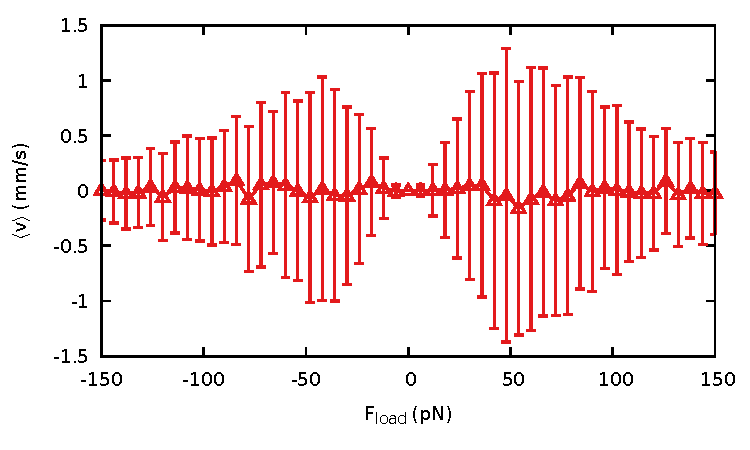
\includegraphics[width=0.45\textwidth,height=!]{tug_F_motor}
\caption{\label{fig:tug_F_motor}
Mean velocity of frustrated motor in between the two filaments under load. 
The variance of the motor's velocity grows as the load increases. 
For even larger loads the motor and filaments start slipping and the variance decreases again.
}
\end{figure}

Although the load is not applied to the motor directly,
there will be a tension on the motor due to interaction with both actin filaments. 
This tension is again given by the difference in the forces applied to their respective ends of the motor,
\begin{equation}
\langle \tau_\text{M} \rangle
= \langle F_{\text{r}_2}\rangle - \langle F_{\text{r}_1}\rangle 
= 2 F_\text{load} - \gamma_\text{A} \left(\langle v_{\text{A}_2}\rangle - \langle v_{\text{A}_1}\rangle \right) .
\label{eq:tension_tug}
\end{equation}
The tension in the motor is shown in figure \ref{fig:tug_F}, 
\begin{figure}[t]
\centering
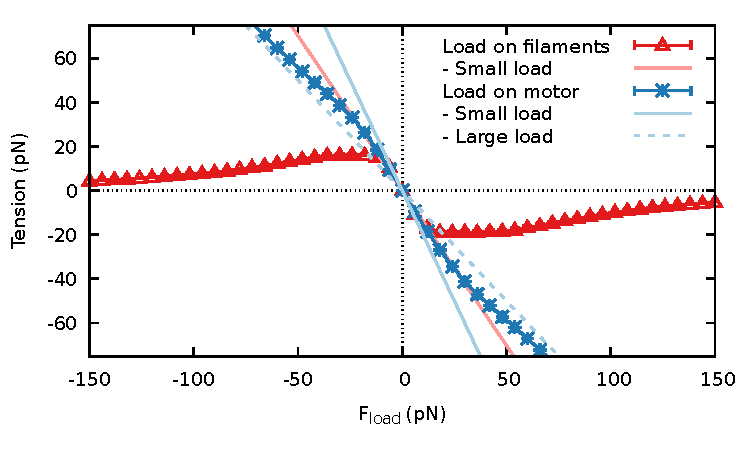
\includegraphics[width=0.45\textwidth,height=!]{tug_F}
\caption{
\label{fig:tug_F}
Tension in the motor, comparison between setup \ref{sec:tug_of_war} with two loaded filaments, setup \ref{sec:load_on_polymer} with one loaded filament and the basic setup with the load on the motor. 
The tension for small loads follows the same trend for the basic setup and ``tug of war'', whereas for large loads the tensions agree for the setups without a load on the motor. 
This is because, only in the case when the load is applied directly on the motor, it remains under the tension even for large loads.
}
\end{figure}
where it is compared to the tension in the setups with only one actin filament.

For small loads, ratchet forces balance the load applied on both filaments, thus the tension is approximately proportional to twice the load 
\[
\langle \tau_\text{M} \rangle \approx 2 F_\text{load} .
\] 
This behavior is similar to the tension in the previously discussed setups  ``load on the motor'' and ``load on the polymer'' setup, cf. equations~\eqref{eq:tension_low_load} and~\eqref{eq:tension_load_on_polymer}, 
where the proportionality constants are $ 1 + \gamma_\text{A} / (\gamma_\text{A} + \gamma_\text{M} )$ and $\gamma_\text{M} / (\gamma_\text{A} + \gamma_\text{M} )$ respectively. 
Note that the proportionality constant for the ``load on the motor'' setup, which lies in the closed interval $[1,2]$, 
is always bigger or equal then the one in the ``load on the polymer'', which is in the interval $[0,1]$, and smaller or equal then in the ``tug of war'' setup. 
This is confirmed by figure~\ref{fig:tug_F}.

As described earlier, the motor starts to slip when the load is increased.
Consequently, the mean ratchet force decreases, cf. figure~\ref{fig:ratchet_force} and~\ref{fig:ratchet_force_decay}, and the increase in tension diminishes, 
as was shown in the figure~\ref{fig:tug_F}.
This behavior underlines the main difference between the ``tug of war'' and ``load on the polymer'' setups and the ``load on the motor'' setup, 
where the load is applied directly to the motor. 
Furthermore, as the ratchet force vanishes for large load, a residual tension from the load remains.
However, in the ``tug of war'' and ``load on the polymer'' setup, this residual tension is not transmitted further to the motor due to the vanishing ratchet interaction.
In the ``load on the polymer'' setup, the tension in the motor does not build up as fast with increasing load because the motor experiences a ratchet force only from one actin filament.
The initial tension there is less then half of the tension in the setup with two loaded filaments.
This suggests that the ratchet force, per motor head, is better transmitted to the motor in the ``tug of war'' setup.


Lastly, the variance of the motor velocity, cf. figure~\ref{fig:tug_F_motor}, seems to behave similarly to the tension on the motor in the figure~\ref{fig:tug_F}. 
While the mean velocity stays close to zero, the variance increases as the tension builds up in the motor. 
As the motor begins to slip over the filaments, the variance appears to decrease again.
However, we do not have a formal proof of this relation.



\subsubsection{Mechanosensing}
\label{sec:mechanosensing}
The last setup, introduced in section~\ref{sec:other_setups}, is the case where the motor is situated between two anti-parallel actin filaments, which are attached to wall via springs, see sketch in figure~\ref{fig:tug}. 
Similarly as in the previous setup, the tension in the motor is given by the difference of the ratchet forces applied on it.
However, in this setup, there is no external load on actin polymers and thus in the steady state we have a simple balance between the ratchet interaction and springs. 
This means that the tension on the motor is given by
\[
\tau_\text{M} 
= \langle F_{\text{r}_2}\rangle - \langle F_{\text{r}_1} \rangle 
= k_\text{sp} \left( \left\langle \Delta x_2 \right\rangle - \left\langle \Delta x_1 \right\rangle \right) ,
\]
where $k_\text{sp}$ is the spring stiffness and $\Delta x_1 = x_1(t) - x_1(0)$ ($\Delta x_2 = x_2(t) - x_2(0)$) is the extension of the spring attached to first (second) actin. 
The tension is plotted in figure~\ref{fig:tug_k} for different stiffnesses $k_\text{sp}$ that represent the varying elasticity of the surrounding network.
\begin{figure}[t]
\centering
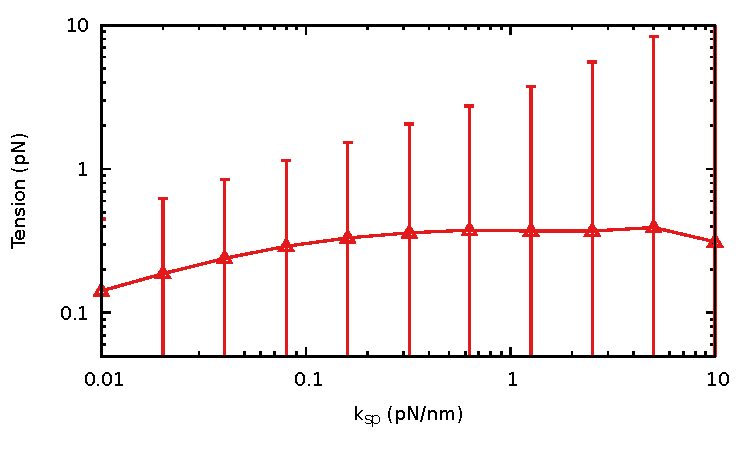
\includegraphics[width=0.45\textwidth,height=!]{tug_k}
\caption{
\label{fig:tug_k}
Mean tension $\langle \tau_\text{M} \rangle$ on the motor for varying spring stiffness $k_\text{sp}$.
Lower stiffness enables the polymers to find a local minimum of the ratchet potential more easily, 
thus the exerted force is lower as the contribution of ratchet potential is minimized. 
On the other hand, high stiffness leads to saturation of the exerted force as the main contribution is given by ratchet potential. 
Inset depicts the mean tension as the function of the spring stiffness on semi-log scale. 
}
\end{figure}
The tension that the motor generates depends strongly on this elasticity $k_\text{sp}$ and saturates for large $k_\text{sp}$. 
This suggests that the motor is not only able to respond to external forces, but also to sense its environment's mechanical properties.

Similar results were obtained for different motor models\cite{stam2015isoforms,albert2014stochastic}. 
However, the models used in those studies exhibit rates that depend on the strain or tension in the myosin motor. 
In our study, we show that this behavior also occurs in a simple Brownian ratchet with constant chemical rates.
It is important to include the fluctuations in this stochastic model to preserve the mechanosensing feature.
In mean field models, where the phenomenological force-velocity relation would be implemented deterministically, 
the motor would essentially stall in this given setup and cease to exert a net force on the filaments. 
Therefore mechanosensing will not occur spontaneously in those models.

It has been shown that mechanosensing takes place on the cellular scale, 
where the cytoskeleton is coupled to the environment through focal adhesions \cite{geiger2009environmental}.

\section{First law of thermodynamics}
\label{sec:energie}
Before we discuss an efficiency of the myosin II motor in various setups,
we need to introduce the basic notions of energy, heat and work. 
We start our discussion from the energy balance on the level of individual trajectories \cite{Pesek2013},
which can be symbolically summarized as 
\begin{equation}
\rmd E = \dbar {\mathcal Q}_\text{M}^\text{hb} + \dbar {\mathcal Q}_\text{A}^\text{hb} + \dbar {\mathcal W}^\text{ext}_\text{M} + \dbar {\mathcal Q}^\text{chem}, 
\label{eq:energy_balance}
\end{equation}
where the energy of the full system consists of the interaction with the ratchet potential~\eqref{eq:ratchet_interaction}
and the energy stored in the ATP molecules that are bound to the motor heads,
\begin{equation}
E( x_\text{M}, x_\text{A}, \{ \zeta_i \}) = V_t( x_\text{M} - x_\text{A} ) + \Delta E \sum\limits_{i=0}^{N-1} \chi( \zeta_i = c ) ,
\label{eq:internal_energy}
\end{equation}
where $\Delta E$ represents the actual internal energy stored by in a single ATP and $\chi$ is a characteristic function\footnote{
$\chi(\text{condition}) = 1$ if condition is fulfilled otherwise $0$.
}.

The energy of the system is subjected to changes driven by the interaction with the environment.
In the case of overdamped diffusion, the environment represents a heath bath
and thus every interaction is associated with a heat exchange \cite{Pesek2013}
\begin{align}
{\mathcal Q}_\text{M}^\text{hb} 
&= \int \rmd x_\text{M} \circ \left[ - \gamma_\text{M} \frac{\rmd x_\text{M} }{\rmd t} + \sqrt{ 2 k_B T \gamma_\text{M} } \, \frac{ \rmd W_\text{M} }{ \rmd t } \right] , 
\label{eq:heat_hb_M} \\
{\mathcal Q}_\text{A}^\text{hb} 
&= \int \rmd x_\text{A} \circ \left[ - \gamma_\text{A} \frac{\rmd x_\text{A} }{\rmd t} + \sqrt{ 2 k_B T \gamma_\text{A} } \, \frac{ \rmd W_\text{A} }{ \rmd t } \right] ,
\label{eq:heat_hb_A}
\end{align} 
where the first term is the dissipation of energy due to the friction and the second is the energy absorbed from the thermal activity of the environment.
Note that those integrals are evaluated in the Stratonovich sense.
The energy is also changed by the work of the external load 
\begin{equation}
{\mathcal W}^\text{ext}_\text{M} = \int \rmd x_\text{M} \circ F_\text{load} = \Delta x_\text{M} F_\text{load}, 
\label{eq:work_load}
\end{equation}
where we use the fact that the external load $F_\text{load}$ is constant. 

The last term in the energy balance \eqref{eq:energy_balance} is the contribution from the chemical cycle. 
The chemical cycle of a motor head, in the most basic form \cite{astumian1996mechanochemical,Bierbaum2011,Bierbaum2013,albert2014stochastic}, is a sequence of binding an ATP molecule, it's hydrolysis, release of phosphor and finally release of ADP.
The first step provides the chemical energy to the system, stored in ATP, while the next steps are associated with dissipation of the remaining energy to surroundings.
Thus the total chemical energy consists of two parts ${\mathcal Q}^\text{chem} = {\mathcal Q}^\text{chem}_\text{in} + {\mathcal Q}^\text{chem}_\text{out}$,
\begin{align}
{\mathcal Q}_\text{in}^\text{chem} 
&= \sum_{t_\text{unbind} \leq t_\text{fin} } \left[ \Delta E + (c-1) V_\text{r}(x_{t_\text{unbind}}) \right] , 
\label{eq:q_in} \\
{\mathcal Q}_\text{out}^\text{chem} 
&= -\sum_{t_\text{bind} \leq t_\text{fin} } \left[ \Delta E + (c-1) V_\text{r}(x_{t_\text{bind}}) \right] 
\label{eq:q_out}
\end{align}
where we sum over the jump times $t_\text{bind}$($t_\text{unbind}$) of all binding(unbinding) events.
$t_\text{fin}$ denotes the duration of the process. 

Figure~\ref{fig:energy_evolution} depicts a time evolution of the internal energy~\eqref{eq:internal_energy} for a single trajectory of the system for $F_\text{load} = 0$.
\begin{figure}
\centering
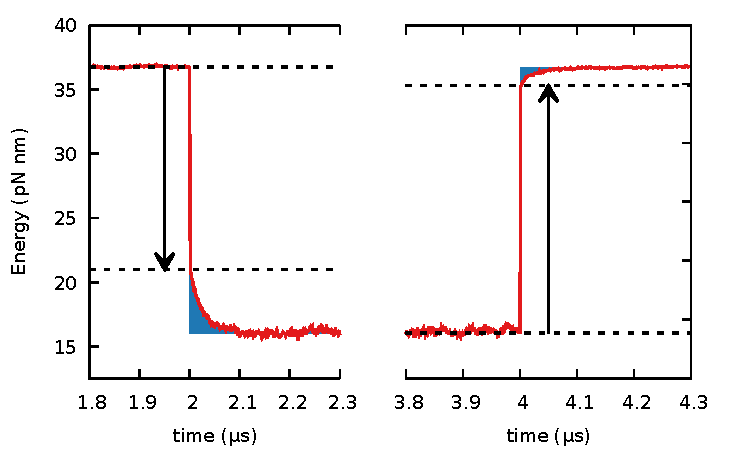
\includegraphics[width=.45\textwidth,height=!]{energy_1head.pdf}
\caption{\label{fig:energy_evolution}
Illustration of the time-evolution of the energy of the system over a single trajectory for $F_\text{load} = 0$.
The red line depicts the internal energy $E$ of the system over the time~\eqref{eq:internal_energy},
black arrows denote the dissipated and obtained chemical heat~\eqref{eq:q_out}, resp.~\eqref{eq:q_in},
and the blue area denote the total heat dissipated to the heat bath ${\mathcal Q}_\text{M}^\text{hb} + {\mathcal Q}_\text{A}^\text{hb}$, 
see~\eqref{eq:heat_hb_M} and~\eqref{eq:heat_hb_A}.
}
\end{figure}
Note, that while we can identify the chemical input and output by the direction of the jump in the total energy, 
without any additional information it is impossible to distinguish which part of the heat dissipated to the heat bath corresponds to myosin or to actin.
For non-zero load, the heat dissipated to the heat bath will contain the work of the external forces as well,
which makes the separation in individual components even more difficult.

\subsection{Load on the motor}
If we restrict the discussion only to the simplest setup, i.e. a single loaded motor with a single actin filament,
and we use the equation of motion~\eqref{eq:eom_M}, 
the heat exchange with the surrounding~\eqref{eq:heat_hb_M} can be rewritten as 
\begin{multline}
{\mathcal Q}_\text{M}^\text{hb} 
= \int \rmd x_\text{M} \circ \left[ \nabla_\text{M} V_t(x_\text{M} - x_\text{A} ) - F_\text{load} \right] 
\\
= \int \rmd x_\text{M} \circ \nabla V_t(x_\text{M} - x_\text{A} ) - {\mathcal W}_\text{M}^\text{ext} ,
\label{eq:heat_hb_M_expl}
\end{multline}
where $\nabla V_t$ denotes the derivative with respect to the argument. 
Similarly for the heat dissipated by actin's interaction with the environment we get 
\begin{multline}
{\mathcal Q}_\text{A}^\text{hb} 
= \int \rmd x_\text{A} \circ \nabla_\text{A} V_t(x_\text{M} - x_\text{A} )
\\
= - \int \rmd x_\text{A} \circ \nabla V_t(x_\text{M} - x_\text{A} ) ,
\label{eq:heat_hb_A_expl}
\end{multline}
thus the heat dissipated to the heath bath can be expressed in terms of the work done by the ratchet potential and external load. 
Consequently, the total energy balance equation~\eqref{eq:energy_balance} simplifies to 
\[
\rmd E 
= \rmd x_\text{M} \circ \nabla_\text{M} V_t  
+ \rmd x_\text{A} \circ \nabla_\text{A} V_t  
+ {\mathcal Q}_\text{in}^\text{chem}
+ {\mathcal Q}_\text{out}^\text{chem} , 
\]
which does not explicitly depend on the load $F_\text{load}$. 

Lastly, in the steady state, 
we can see that the excess of the chemical cycle in the steady state is dissipated as the work of ratchet potential~\eqref{eq:ratchet_potential} over the separation of motor and filament 
\begin{multline}
\left\langle 
{\mathcal Q}_\text{in}^\text{chem} + {\mathcal Q}_\text{out}^\text{chem} 
\right\rangle 
\\
= 
\left\langle 
\int \rmd \left( x_\text{M} - x_\text{A} \right) \circ \left[ - \nabla V_t( x_\text{M} - x_\text{A} ) \right]
\right\rangle ,
\label{eq:chemical_excess}
\end{multline} 
which can be further interpreted in terms of tension on the polymer $\tau_\text{A}$, cf.~\eqref{eq:tension_on_polymer}, and the relative velocity $v$ 
\begin{equation}
\left\langle 
{\mathcal Q}_\text{in}^\text{chem} + {\mathcal Q}_\text{out}^\text{chem} 
\right\rangle 
= - \left\langle \int \rmd t \; v \, \tau_\text{A} \right\rangle .
\label{eq:excess_heat} 
\end{equation}
%TODO reference previous text 

\subsection{Heat fluxes}
Furthermore, note that the internal energy of the system~\eqref{eq:internal_energy} is bounded.
Hence, if we interpret the energy balance equation~\eqref{eq:energy_balance} in terms of mean dissipation rates defined as 
\begin{equation}
q = \lim_{\Delta t \to \infty} \frac{1}{\Delta t} \left\langle {\mathcal Q}(\Delta t) \right\rangle ,
\label{eq:heat_flux}
\end{equation}
we obtain an equation representing the conservation of fluxes 
\begin{equation}
0 = q_\text{M}^\text{hb} + q_\text{A}^\text{hb} + w^\text{ext}_\text{M} + q^\text{chem} 
\label{eq:heat_flux_balance}
\end{equation}
for arbitrary initial condition. 
Such equality is trivially true for arbitrarily small times when the initial condition corresponds to the steady state.


\subsection{Other setups} 
In section \ref{sec:ratchet} we introduced two alternative models, more suitable for capturing the behavior of myosin motors inside the polymer network known as the actomyosin cortex.

\subsubsection{Load on the polymer}
The ``load on the polymer'' setup is a variation to the ``load on the motor'' setup, cf. section~\ref{sec:load_on_polymer}. 
From the mathematical perspective, it is identical to the ``load on the motor'' setup although differently interpreted. 
What was called motor in the basic setup, is now called polymer and visa versa.
This means that energy balance~\eqref{eq:energy_balance} is preserved 
with basic expressions for heat dissipated to the heat bath~\eqref{eq:heat_hb_M} and~\eqref{eq:heat_hb_A} kept intact 
and external work on the motor ${\mathcal W}_\text{M}^\text{ext}$ replaced by the external work on the polymer
\[
{\mathcal W}_\text{A}^\text{ext} = - \int \rmd x_\text{A} \circ F_\text{load} = - \Delta x_\text{A} \, F_\text{load} . 
\]
Note, that in this particular setup the load is applied in the opposite direction, as can be seen from the equations of motion~\eqref{eq:eom_A_lp}. %TODO check if true 

Similarly expressions~\eqref{eq:heat_hb_M_expl} and~\eqref{eq:heat_hb_A_expl} are modified to
\begin{align*}
{\mathcal Q}_\text{M}^\text{hb} 
&= - \int \rmd x_\text{M} \circ \nabla V_t(x_\text{A} - x_\text{M} ) ,
\\
{\mathcal Q}_\text{A}^\text{hb} 
&= \int \rmd x_\text{A} \circ \nabla V_t(x_\text{A} - x_\text{M} ) - {\mathcal W}_\text{A}^\text{ext} .
\end{align*} 
Consequently the excess of the chemical cycle~\eqref{eq:chemical_excess} changes to 
\begin{multline*}
\left\langle 
{\mathcal Q}_\text{in}^\text{chem} + {\mathcal Q}_\text{out}^\text{chem} 
\right\rangle 
\\
= 
\left\langle 
\int \rmd \left( x_\text{M} - x_\text{A} \right) \circ \left[ - \nabla V_t( x_\text{A} - x_\text{M} ) \right]
\right\rangle ,
\end{multline*} 
which can be again interpreted in terms of the relative velocity $v$ and the tension on the motor $\tau_\text{M}$, cf.~\eqref{eq:tension_load_on_polymer},  
\begin{equation}
\left\langle 
{\mathcal Q}_\text{in}^\text{chem} + {\mathcal Q}_\text{out}^\text{chem} 
\right\rangle 
= \left\langle \int \rmd t \; v \, \tau_\text{M} \right\rangle .
\label{eq:chemical_excess_poly}
\end{equation}

\subsubsection{Tug of war}
In the ``tug of war'' setup, see section~\ref{sec:tug_of_war} and figure~\ref{fig:tug_F_illustration},
the motor is placed between two polymers on which the load is applied,
hence the energy balance~\eqref{eq:energy_balance} is modified to  
\begin{multline}
\rmd E = \dbar {\mathcal Q}_\text{M}^\text{hb} + \dbar {\mathcal Q}_{\text{A}_1}^\text{hb} + \dbar {\mathcal Q}_{\text{A}_2}^\text{hb} 
\\
+ \dbar {\mathcal W}^\text{ext}_{\text{A}_1} + \dbar {\mathcal W}^\text{ext}_{\text{A}_2} + \dbar {\mathcal Q}^\text{chem}, 
\label{eq:energy_balance_two_filaments}
\end{multline}
where the energy now contains contributions from both polymers
\begin{multline*}
E( x_\text{M}, x_{\text{A}_1}, x_{\text{A}_2}, \{ \zeta_i \}) 
= V_t( x_\text{M} - x_{\text{A}_1} ) 
\\
+ V_t( x_{\text{A}_2} - x_\text{M} ) 
+ \Delta E \sum\limits_{i=0}^{N-1} \chi( \zeta_i = c ) .
\end{multline*}
Note, that the last sum is over all heads of the motor, $N = N_{\text{A}_1} + N_{\text{A}_2}$.
Contributions from the heat exchange with the environment~\eqref{eq:heat_hb_A} remain the same, even though in this case we have two contributions from both filaments
\begin{align*}
{\mathcal Q}_{\text{A}_1}^\text{hb} 
&= \int \rmd x_{\text{A}_1} \circ \left[ - \gamma_\text{A} \frac{\rmd x_{\text{A}_1} }{\rmd t} + \sqrt{ 2 k_B T \gamma_\text{A} } \, \frac{ \rmd W_{\text{A}_1} }{ \rmd t } \right] , \\ 
{\mathcal Q}_{\text{A}_2}^\text{hb} 
&= \int \rmd x_{\text{A}_2} \circ \left[ - \gamma_\text{A} \frac{\rmd x_{\text{A}_2} }{\rmd t} + \sqrt{ 2 k_B T \gamma_\text{A} } \, \frac{ \rmd W_{\text{A}_2} }{ \rmd t } \right] ,
\end{align*}
and the external load is now not applied on the motor but on each actin polymer.
Hence, equation~\eqref{eq:work_load} is replaced by
\begin{align*}
{\mathcal W}^\text{ext}_{\text{A}_1} &= \int \rmd x_{\text{A}_1} \circ F_\text{load} = \Delta x_{\text{A}_1} F_\text{load}, 
\\
{\mathcal W}^\text{ext}_{\text{A}_2} &= - \int \rmd x_{\text{A}_2} \circ F_\text{load} = - \Delta x_{\text{A}_2} F_\text{load}. 
\end{align*}

Note, that the interpretation of the energy balance \eqref{eq:energy_balance_two_filaments} in terms of the heat fluxes \eqref{eq:heat_flux}
while following the same arguments as for \eqref{eq:heat_flux_balance} is possible and leads to   
\[
0 = q_\text{M}^\text{hb} + q_{\text{A}_1}^\text{hb} + q_{\text{A}_2}^\text{hb} + w^\text{ext}_{\text{A}_1} + w^\text{ext}_{\text{A}_2} + q^\text{chem} .
\]

Similarly to the ``load on the motor'' setup, we can express the excess from the chemical cycle in the steady state as sum of work by the ratchet forces with respect to their respective displacements,
\begin{multline}
\left\langle 
{\mathcal Q}_\text{in}^\text{chem} + {\mathcal Q}_\text{out}^\text{chem} 
\right\rangle 
\\
= 
\left\langle 
\int \rmd \left( x_\text{M} - x_{\text{A}_1} \right) \circ \left[ - \nabla V_t( x_\text{M} - x_{\text{A}_1} ) \right]
\right\rangle 
\\
+
\left\langle 
\int \rmd \left( x_\text{M} - x_{\text{A}_2} \right) \circ \left[ - \nabla V_t( x_{\text{A}_2} - x_\text{M} ) \right]
\right\rangle .
\label{eq:excess_heat_tug}
\end{multline} 
If we assume that displacements in the respective integrals are typically anti-symmetric, due to the anti-symmetry of the setup, 
we can interpret the excess chemical heat as a covariance of the tension on the motor~\eqref{eq:tension_tug} with the relative velocity of the motor with respect to a single polymer integrated over the time, 
as in the equation~\eqref{eq:excess_heat}. 
Note, that in this particular setup the interpretation in terms of the tension is not so straightforward as in the case of the setup with either ``load on the motor'' or ``load on the polymer'', 
because the individual displacements $x_\text{M} - x_{\text{A}_1}$ and $x_\text{M} - x_{\text{A}_2}$ are not independent nor dependent only on very short time scales.
Only in the long time regime they are anti-symmetric. 


\subsubsection{Elastic environment}
\label{sec:power_elastic}
Another model, described in paragraph~\ref{sec:environment} and depicted in figure~\ref{fig:tug}, 
further modifies the energy balance~\eqref{eq:energy_balance}, resp.~\eqref{eq:energy_balance_two_filaments},
\begin{equation*}
\rmd E = \dbar {\mathcal Q}_\text{M}^\text{hb} + \dbar {\mathcal Q}_{\text{A}_1}^\text{hb} + \dbar {\mathcal Q}_{\text{A}_2}^\text{hb} + \dbar {\mathcal Q}^\text{chem}, 
\end{equation*}
as there is no external load but all the accumulated energy is now stored in harmonic potentials 
\begin{multline*}
E( x_\text{M}, x_{\text{A}_1}, x_{\text{A}_2}, \{ \zeta_i \}) 
= V_t( x_\text{M} - x_{\text{A}_1} ) 
+ V_t( x_{\text{A}_2} - x_\text{M} ) 
\\
+ \frac{1}{2} k_\text{sp} \left[ x_{\text{A}_1} - x_{\text{A}_1}(0) \right]^2 
+ \frac{1}{2} k_\text{sp} \left[ x_{\text{A}_2} - x_{\text{A}_2}(0) \right]^2 
\\
+ \Delta E \sum\limits_{i=0}^{N-1} \chi( \zeta_i = c ) .
\end{multline*}
Contrary to the previous setup, the total energy of the system is no longer bound, hence the heat fluxes~\eqref{eq:heat_flux} are only balanced in the steady state.

Lastly we again look at the excess output from the chemical cycle
\begin{multline*}
\left\langle 
{\mathcal Q}_\text{in}^\text{chem} + {\mathcal Q}_\text{out}^\text{chem} 
\right\rangle 
\\
= 
\left\langle 
\int \rmd \left( x_\text{M} - x_{\text{A}_1} \right) \circ \left[ - \nabla V_t( x_\text{M} - x_{\text{A}_1} ) \right]
\right\rangle 
\\
+
\left\langle 
\int \rmd \left( x_\text{M} - x_{\text{A}_2} \right) \circ \left[ - \nabla V_t( x_{\text{A}_2} - x_\text{M} ) \right]
\right\rangle 
\\
+ k_\text{sp} \left\langle \int \rmd x_{\text{A}_1} \circ \left( x_{\text{A}_1} - x_{\text{A}_1}(0) \right) \right\rangle
\\ 
+ k_\text{sp} \left\langle \int \rmd x_{\text{A}_2} \circ \left( x_{\text{A}_2} - x_{\text{A}_2}(0) \right) \right\rangle
,
\end{multline*} 
which further simplifies to 
\begin{multline*}
\left\langle 
{\mathcal Q}_\text{in}^\text{chem} + {\mathcal Q}_\text{out}^\text{chem} 
\right\rangle 
\\
= 
\left\langle 
\int \rmd \left( x_\text{M} - x_{\text{A}_1} \right) \circ \left[ - \nabla V_t( x_\text{M} - x_{\text{A}_1} ) \right]
\right\rangle 
\\
+
\left\langle 
\int \rmd \left( x_\text{M} - x_{\text{A}_2} \right) \circ \left[ - \nabla V_t( x_{\text{A}_2} - x_\text{M} ) \right]
\right\rangle 
\\
+ \left\langle 
\Delta E^\text{sp}_1 
\right\rangle
+ \left\langle 
\Delta E^\text{sp}_2 
\right\rangle ,
\end{multline*} 
where $E^\text{sp}$ denote the energy stored in the spring, i.e. 
\[
\left\langle \Delta E^\text{sp}_{1/2} \right\rangle 
= 
\frac{1}{2} k_\text{sp}
\left\langle
\left( 
x_{\text{A}_{1/2}}(t) 
- 
x_{\text{A}_{1/2}}(0)  
\right)^2 
\right\rangle
.
\]
The interpretation of this excess chemical energy in terms of the tension is even more difficult than in the ``tug of war'' setup~\eqref{eq:excess_heat_tug} due to multiple factors.
First, there are additional terms related to the change of the energy of springs.
Second, the mean velocity of all elements in the steady state is zero due to the anti-symmetry of the setup and no additional external force breaking this symmetry. 
Hence the argument about long time regime is invalid in this case.
And lastly, no other additional information is known about correlations in the displacement with respect to the motor. 


\section{Efficiency} 
\label{sec:efficiency}
In previous years, a lot of effort was directed towards the assessment of the efficiency of molecular motors \cite{Schmiedl2008,boksenbojm2009entropy}. %TODO more citations
Unfortunately, main focus of these works was biased towards the transport properties of the aforementioned motors. 
However the main role of myosin II is generating the tension in the cytoskeletal network \cite{ma2012nonmuscle,chugh2017actin,monier2010actomyosin}.

Efficiency, in general, relates a ``useful'' output to the input.
As what is considered ``useful'' heavily depends on the setup, there is a plethora of possible choices.
Here we discuss a commonly made choice and one particular choice which is, to the best knowledge of the authors, previously not discussed in the literature. 
First, we revisit the most common definition of efficiency, well discussed in the literature \cite{}, which is related to the transport properties of molecular motors. %TODO cite
The second definition of the chemical efficiency captures the speed of the tension generation in networks, due to myosin~II. %TODO correlates velocity with tension

\subsection{Transport efficiency} 
As we have stated, the first efficiency we discuss is related to transport properties. 
Namely, we identify the heat dissipated to the environment by the motor alone as the output work 
\[
{\mathcal W}^\text{out}_\text{M} = - {\mathcal Q}^\text{hb}_\text{M} 
\] 
and chemical work $\mathcal Q^\text{chem}$ and the work done by the load $\mathcal W^\text{ext}_\text{M}$.
Hence the transport efficiency can be defined as 
\[
\eta_\text{tr} = \frac{ \left\langle {\mathcal W}^\text{out}_\text{M} \right\rangle }{ \left\langle {\mathcal Q}^\text{chem} \right\rangle + \left\langle {\mathcal W}^\text{ext}_\text{M} \right\rangle } .
\]
Note, that for a large load ($F_\text{load} \to \infty$) such efficiency approaches $\eta_\text{tr} \to 1$, 
while in absence of a load $F_\text{load} = 0$ it captures how much of the chemical energy is dissipated by the motor's motion  
\[
\eta_\text{tr}( F_\text{load} = 0 ) = \frac{ \left\langle \int \rmd x_\text{M} \circ \left[ - \nabla_\text{M} V_t \right] \right\rangle }{ \left\langle {\mathcal Q}^\text{chem} \right\rangle } ,
\]
i.e. how much of the chemical energy provided to the system is dissipated by the motor and not by the polymer. 


\subsection{Chemical efficiency} %TODO 
\label{sec:chemical_efficiency}
An alternative approach is to identify the ``useful'' output by looking at the chemical energy, supplied by ATP, that is transformed to other forms of energy, 
i.e. either it is dissipated by myosin and actin through their diffusion or it is stored in the interaction potential and thus increases the tension in the system. 
This consideration leads to a chemical efficiency defined as 
\begin{equation}
\eta_\text{chem} = \frac{\langle\mathcal Q^\text{chem}_\text{in}\rangle+\langle\mathcal Q^\text{chem}_\text{out}\rangle}{\langle\mathcal Q^\text{chem}_\text{in}\rangle} .
\label{eq:efficiency}
\end{equation}

\subsubsection{Load on the motor}
For a system where the load is applied on the four headed motor, we investigate the dependency of such chemical efficiency on the load, see figure~\ref{fig:chem}.
We observe that the chemical efficiency has two local maximums. 
We will later show that these two maximums correspond to a frustrated system, 
where the load is close to the point where it is able to overcome any force induced by the ratchet potential. 
Another observation, which we will discuss in depth later, is that the efficiency reaches negative values for large loads, 
which we interpret as work done by the load $F_\text{load}$ that is converted back to chemical energy. 
\begin{figure}[t]
\centering
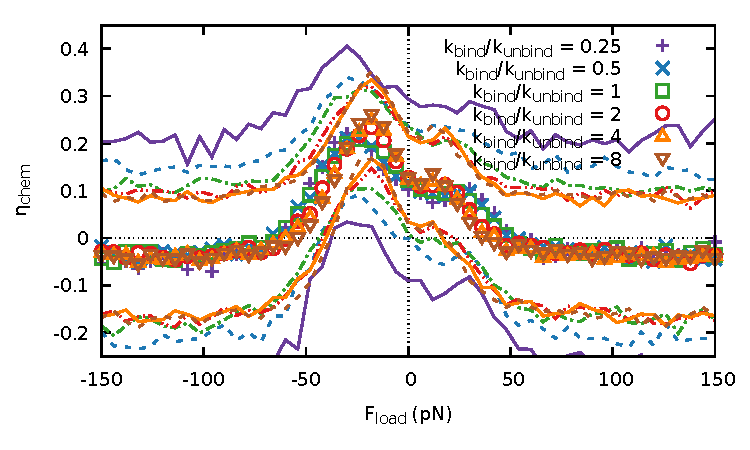
\includegraphics[width=0.45\textwidth,height=!]{chemical_cycle}
\caption{
\label{fig:chem}
Chemical efficiency $\eta$ as a function of load force $F_\text{load}$.
Solid lines are plotted at the level of $1\sigma$. 
By increasing the $k_d/k_a$ ratio the local maximums of chemical efficiencies are getting closer to the origin,
and their fluctuations decrease. 
}
\end{figure}

In order to properly understand these features, 
we try to evaluate the chemical efficiency \eqref{eq:efficiency} in a steady state. 
We start by evaluating the mean heat \eqref{eq:q_in} and \eqref{eq:q_out} produced over a time interval of length $\Delta t$ 
by transitions of a single head $i$ displaced with respect to the end of the motor by $i d$,  
\begin{gather*}
\begin{multlined}[b][.42\textwidth]
\langle \mathcal Q^\text{chem}_\text{in}(i) \rangle 
= \Delta t \, k_\text{unbind} 
\\ \times 
\!\!\!\! \sum\limits_{\{\zeta_j\} : \zeta_i = 1 } \!\!\!\! \rho(\{ \zeta_j \} ) 
\left[ \Delta E - (1-c) \left\langle V_\text{r}(x - i \, d ) \middle| \{ \zeta_j \} \right\rangle \right] 
\end{multlined}
%\label{eq:mean_q_in} 
\\
\begin{multlined}[b][.42\textwidth]
\langle \mathcal Q^\text{chem}_\text{out}(i) \rangle 
= - \Delta t \, k_\text{bind} 
\\ \times 
\!\!\!\! \sum\limits_{\{\zeta_j\} : \zeta_i = c } \!\!\!\! \rho(\{ \zeta_j \} ) 
\left[ \Delta E - (1-c) \left\langle V_\text{r}(x - i \, d ) \middle| \{ \zeta_j \} \right\rangle \right] 
\end{multlined}
%\label{eq:mean_q_out}
\end{gather*}
where $\langle V | X \rangle$ is the steady state conditional mean value with respect to the fixed internal state $X$ 
and $\rho(X) \in [0,1]$ denotes the probability of the occupation of the corresponding internal state $X$ in the steady state, 
which does not depend on the position due to the independence of the internal state dynamics~\eqref{eq:transition} on position. 
Moreover, due to the independence of individual heads the probability occupation of a given internal state can be written as 
\[
\rho( \{ \zeta_i \} ) = \prod_{i=0}^{N-1} \rho_1( \zeta_i ), 
\]  
where 
\[
\rho_1(\zeta) = \begin{cases} 
\frac{ k_\text{bind} }{ k_\text{bind} + k_\text{unbind} } & \zeta = 1 , \\
\frac{ k_\text{unbind} }{ k_\text{bind} + k_\text{unbind} } & \zeta = c . 
\end{cases} 
\]

Another consequence of the independence of the individual heads 
is that we can express the total mean heats produced in the chemical cycle as a sum of contributions from individual heads
\begin{align*}
\langle \mathcal Q_\text{in}^\text{chem} \rangle 
=& \sum\limits_{i=0}^{N-1} \left\langle \mathcal Q_\text{in}^\text{chem}(i) \right\rangle 
= \Delta t \frac{ k_\text{bind} k_\text{unbind} }{ k_\text{bind} + k_\text{unbind} } 
\\ &\times
\left[ N \, \Delta E 
- (1-c) \sum\limits_{i=0}^{N-1} \left\langle V_\text{r}(x - i d ) \middle| \zeta_i = 1 \right\rangle 
\right] ,  
\\
\langle \mathcal Q^\text{chem}_\text{out} \rangle 
=& \sum\limits_{i=0}^{N-1} \left\langle \mathcal Q_\text{out}^\text{chem}(i) \right\rangle 
= - \Delta t \frac{ k_\text{bind} k_\text{unbind} }{ k_\text{bind} + k_\text{unbind} } 
\\ &\times
\left[ N \, \Delta E 
- (1-c) \sum\limits_{i=0}^{N-1} \left\langle V_\text{r}(x - i d ) \middle| \zeta_i = c \right\rangle  
\right] , 
\end{align*}
which leads to a more explicit expression for the efficiency \eqref{eq:efficiency} 
\begin{multline*}
\eta_\text{chem} = \frac{1-c}{N}
\\ \times
\sum\limits_{i=0}^{N-1} \frac{ \left\langle V_\text{r}(x-id) \middle| \zeta_i = c \right\rangle - \left\langle V_\text{r}( x -id ) \middle| \zeta_i = 1 \right\rangle }
{ \Delta E - \frac{1-c}{N} \sum\limits_{j=0}^{N-1} \left\langle V_\text{r}(x-jd) \middle| \zeta_j = 1 \right\rangle } 
. 
\end{multline*}
We can further introduce an average probability density over all heads 
\begin{equation}
\bar{\rho}(x,\zeta) = \frac{1}{N} \sum\limits_{i=0}^{N-1} \sum\limits_{ \{ \zeta_j \} : \zeta_i = \zeta } \rho( x + i d, \{ \zeta_j \} ) ,
\label{eq:eff_distribution}
\end{equation}
and consequently the conditional average probability density
\begin{equation}
\bar{\rho}(x|\zeta) = \bar{\rho}(x,\zeta) \left[ \int\limits_0^\ell \rmd y \; \bar{\rho}(y,\zeta) \right]^{-1}
\label{eq:cond_prob}
\end{equation}
which allow us to further simplify the expression for the chemical efficiency to 
\begin{equation}
\eta_\text{chem} = (1-c)
\frac{ \left\langle V_\text{r}(x) \middle| \zeta = c \right\rangle_{\bar{\rho}} - \left\langle V_\text{r}(x) \middle| \zeta = 1 \right\rangle_{\bar{\rho}} }
{ \Delta E - (1-c) \left\langle V_\text{r}(x) \middle| \zeta = 1 \right\rangle_{\bar{\rho}} } 
. 
\label{eq:eta}
\end{equation}
We can see that the numerator is given by the average difference between mean potentials in the ATP attached and detached states over all heads. 
As the potential is known in our model, the only missing information is thus the steady state distribution 
or to be more precise the average steady state density for all heads \eqref{eq:eff_distribution}.  
These distributions are empirically obtained by collecting the positions of the heads over all times in which the head was in the ATP bound/unbound state.
They are shown in figure~\ref{fig:pos_distr} for different load forces. 
\begin{figure}[t]
\centering
\subfigure[ATP unbound state]{ 
\centering
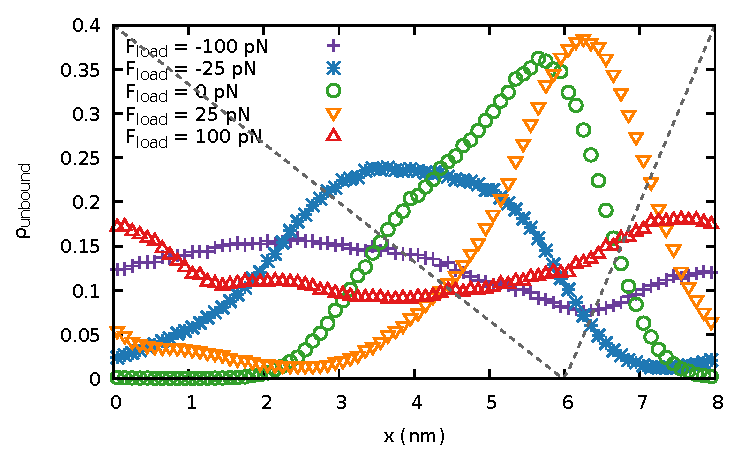
\includegraphics[width=.45\textwidth,height=!]{pos_distr_a_F}
}
\\
\subfigure[ATP bound state]{
\centering
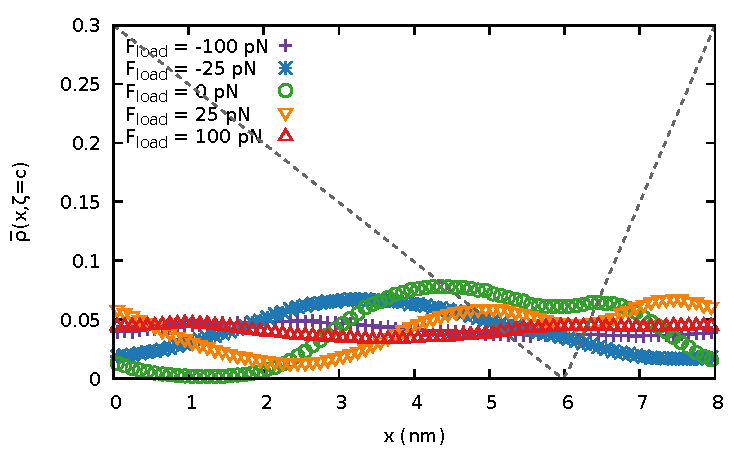
\includegraphics[width=.45\textwidth,height=!]{pos_distr_d_F}
}
\caption{
\label{fig:pos_distr}
Spatial distributions $\rho$ of the motor heads with respect to the ratchet potential (denoted by dashed black line) for different load forces $F_\text{load}$.
The spatial distribution is taken as the average over all heads of a given motor in a given internal state.
We observe that heads in the ATP unbound state follow the potential closely while those in the bound state do not. 
Also by increasing the external load, all distributions universally become flat. 
}
\end{figure}

The difference between the average distribution \eqref{eq:eff_distribution} in the ATP bound state and ATP unbound state is directly translated to the mean heat flux \eqref{eq:heat_flux} out of the chemical system
\begin{multline}
q_\text{in}^\text{chem} + q_\text{out}^\text{chem} 
= (1-c) \frac{ k_\text{bind} k_\text{unbind} }{ k_\text{bind} + k_\text{unbind} } 
\\ \times
\left[ \left\langle V_\text{r}(x) \middle| \zeta = c \right\rangle_{\bar{\rho}} - \left\langle V_\text{r}(x) \middle| \zeta = 1 \right\rangle_{\bar{\rho}} \right] ,
\label{eq:heat_flux_explicit}
\end{multline} 
which is depicted in the figure~\ref{fig:chem_energy_distr}, 
\begin{figure}[t]
\centering
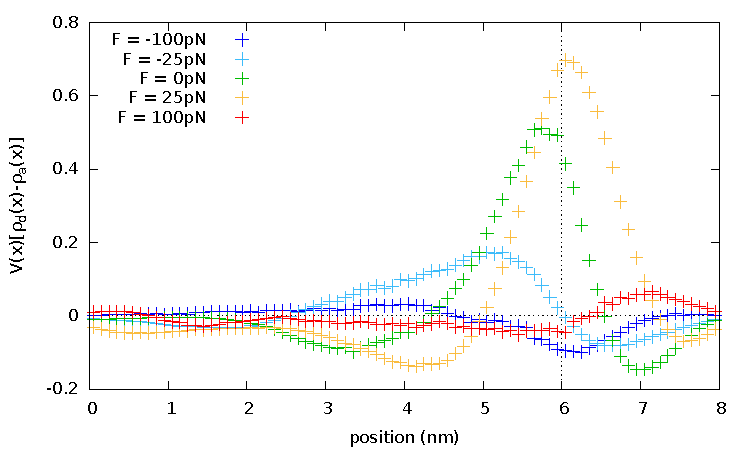
\includegraphics[width=0.45\textwidth,height=!]{chem_energy_distr_all_F}
\caption{
\label{fig:chem_energy_distr}
Heat flux~\eqref{eq:heat_flux_explicit} density, i.e. $\int \rmd x \; q(x) = q$, for various loads.  
We can see that the largest heat flux is around the ratchet potential~\eqref{eq:ratchet_potential} minimum, where the gap is largest. 
However, the region which contributes to the chemical efficiency~\eqref{eq:eta} the most is the close to the ratchet potential maximum, 
see figure~\ref{fig:chem_efficiency_distr} where the heat flux is very small. 
}
\end{figure}
where we show the spatial dependency of the heat fluxes.
We can see that a major flux is close to the ratchet potential's minimum \eqref{eq:ratchet_potential} where both the probability density is localized and the gap is the largest. 
On the other hand, close to the ratchet potential's maximum the heat flux is close to zero.
However, if we compare it to the numerator of the chemical efficiency~\eqref{eq:eta}, see figure~\ref{fig:chem_efficiency_distr}, 
\begin{figure}[t]
\centering
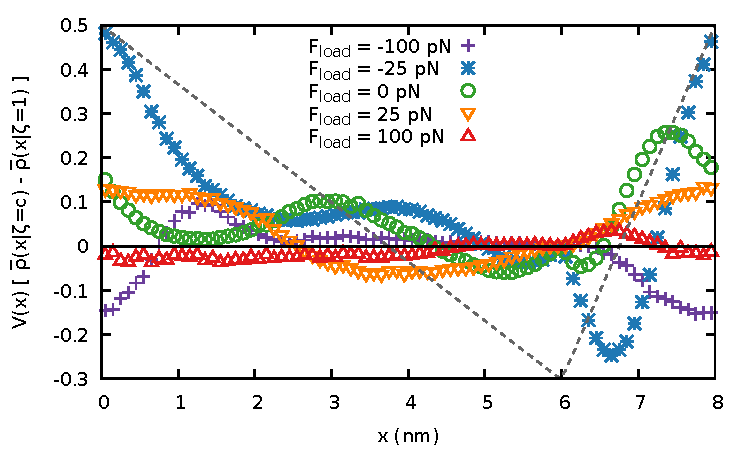
\includegraphics[width=0.45\textwidth,height=!]{chem_efficiency_distr_all_F}
\caption{
\label{fig:chem_efficiency_distr}
Space resolved numerator of the efficiency \eqref{eq:eta} for various load forces $F_\text{load}$. 
We observe that the optimal output is achieved when there is the biggest discrepancy between spatial distributions, compare with figure~\ref{fig:pos_distr} and \ref{fig:chem}. 
}
\end{figure}
we can see that a major contribution to the chemical efficiency actually comes from the region around the ratchet potential's maximum.
This discrepancy can be interpreted in the following sense: 
While most transitions occur close to the ratchet potential's minimum due to the large probability density, thus providing a large flux, 
those particles after a transition does not diffuse far before next transition, 
hence the contribution to the chemical efficiency, associated with the discrepancy between chemical input and output, is relatively small. 
On the other hand, a particle that switched its internal state close to the potential maximum relaxes relatively fast, compared to the transition rates, 
to the vicinity of the ratchet potential's minimum and thus creates a larger discrepancy leading to high contribution to the efficiency. 
However these transitions are rare due to the low probability density and hence the total flux density is relatively small.  

In absence of an external load, $F_\text{load}=0$, 
the maximum of the distribution, see fig.~\ref{fig:pos_distr}, is close to the minimum of the potential,  
where the discrepancy in the position comes from the averaging over multiple heads with a fixed distance between them, 
which does not match with the period of the ratchet potential. 
Also the fact that the distributions seem to exhibit multiple peaks, can be attributed to the motor having four heads. 
Both in the bound and unbound state, the head can be found predominantly on the ``soft'' slope of the ratchet.

When the load is increased to $F_\text{load} = 25 \, \mathrm{pN}$, the average steady state distribution shifts to the right in both the ATP bound and unbound state. 
While the distribution for the ATP unbound state remains peaked around the potential minimum, cf. figure~\ref{fig:pos_distr},
the distribution in the ATP bound state flattens out and increases around the potential maximum. 
This is due to the potential being less steep, which means that heads in that particular state are more susceptible to external forces,  
which in this particular case leads to an increase of $\eta$ due to the increase in discrepancy between the average distributions, 
see figures~\ref{fig:chem} and \ref{fig:chem_energy_distr}. 

For a load in the opposite direction $F_\text{load}= -25 \, \mathrm{pN}$ the effect on average densities is similar but less pronounced, 
see figure~\ref{fig:chem_energy_distr}, 
since the slope of the ratchet on the side is less steep and the distributions get more spread out, cf. figure~\ref{fig:pos_distr}. 

For larger loads, distributions shift and flatten even more, figure~\ref{fig:pos_distr}. 
In the extreme situation, it leads to completely flat distribution and thus zero efficiency, figure~\ref{fig:chem}.
For high loads we also observe a population inversion, see figure~\ref{fig:pos_distr}, 
where the potential maximum is more occupied then the potential minimum. 
This is due to the effective friction caused by the potential. 
As the particle gets slower when dragged along the potential gradient, 
 they spend more time on the up-slope then on the down-slope of the potential.
Such behavior is associated with a negative efficiency. 
In the appendix we have proven this hypothesis on the system with a single head and have shown that the efficiency decay with the force 
\[
\eta \asymp - \frac{1}{ F_\text{load}^2 } \qquad \text{for} \quad F_\text{load} \to \pm \infty .
\]

\subsubsection{Dependency on number of heads}
If we interpret the dependency of the chemical efficiency \eqref{eq:eta} on the load as a probabilistic distribution with finite variance and assume that the main contribution to the shape, figure~\ref{fig:chem}, is from the numerator, 
by using central limit theorem the efficiency-load dependency will approach a Gaussian distribution with increasing number of heads. 
This is confirmed by figure~\ref{fig:chem_eff_1head}, where indeed the distribution is getting broader with increasing number of heads and has only a single maximum.
\begin{figure}[t]
\centering
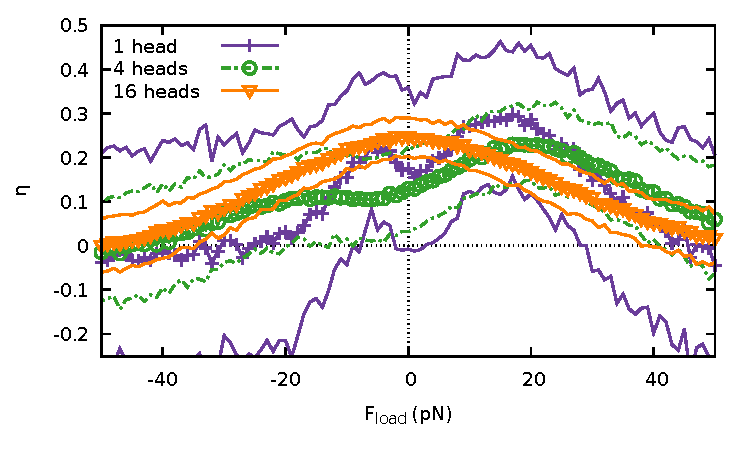
\includegraphics[width=0.45\textwidth,height=!]{chemical_cycle_1head}
\caption{
\label{fig:chem_eff_1head}
Chemical efficiency of a motor under load with variable number of motor's heads.
The ``solid'' lines are drawn on the level of one sigma. 
We observe that with increasing number of heads the efficiency \eqref{eq:efficiency} distribution gets broader and it's variance decreases.
Moreover, for sixteen heads it became centered without two local maximums.
}
\end{figure}
It is also apparent that there is no qualitative difference in chemical efficiency between the system with four heads and one head.
Moreover we can see that the empirical efficiency has a smaller variance with the increasing number of heads. 
From these we can conclude that there is a significant qualitative difference between motors with low and high numbers of heads. 
Thus experiments in vitro with large myosin II motors \cite{} does not necessarily capture the behavior of the motors inside a cytoskeleton. %TODO cite

\subsubsection{Local minimum}
Another trait of the chemical efficiency curves are the local minimums around $F_\text{load}=0$. 
This can be understood from equation \eqref{eq:eta}, which is determined by the ratchet potential averaged with the heads' distribution in the attached and detached state. 
For a one headed motor, these distribution will both be peaked around the minimum of the ratchet potential. 
In fact, these distributions will be given by the Boltzmann distribution
\begin{equation}
\rho_0(x,\zeta) = \frac{1}{Z(\zeta)} e^{-\beta \zeta V_\text{r}(x)}
\end{equation} 
in the lowest order of approximation, as the binding and unbinding rates operate on much longer time scale then the relaxation governed by the diffusion. 
From this point of view, ATP binding is effectively equivalent to an increasing of the temperature of the heat bath $T\rightarrow\frac{T}{c}$. 
Hence the distributions for the ATP bound state are broader and the expectation value of $V_\text{r}$ will be bigger than in the attached state and $\eta$ will be positive. 

Now if we apply a small external force, those distributions will be slightly perturbed. 
Following the McLennan formula~\cite{} we obtain %TODO 
\begin{align*}
\rho^*(x) 
&\sim e^{-\beta \left[V_\text{r}(x) - F_\text{load} \left( x - x_\text{min} \right) \right]} \\
&\approx \rho_0(x) \left[1 + \beta F_\text{load} \left( x - x_\text{min} \right) \right]
\end{align*}
close to the potential minimum $x_\text{min}$, i.e. $V(x) \ge V(x_\text{min})$. 
This leads, for small $F_\text{load}$, to a shift of the distribution $\rho$ in the direction of the load
as can be seen from 
\begin{multline}
\left\langle x \right\rangle_{\rho^*} 
= x_\text{min} + \left\langle x - x_\text{min} \right\rangle_{\rho^*}
\\
\approx x_\text{min} + \left\langle x - x_\text{min} \right\rangle_{\rho_0} 
+ \beta F \left\langle \left( x - x_\text{min} \right)^2 \right\rangle_{\rho_0} 
\\
= \left\langle x \right\rangle_{\rho_0}
+ \beta F \left\langle \left( x - x_\text{min} \right)^2 \right\rangle_{\rho_0} .
\label{eq:mean_position_shift}
\end{multline}
From the previous equation it follows that a more spread-out distribution will be affected more by the force.
This means that in our case the ATP bound state will be more affected.
A larger displacement of the distribution, away from the potential's minimum, 
means that the mean ratchet potential in the ATP bound state $\left\langle V_\text{r} \middle| \zeta = c \right\rangle$ will increase more than the mean ratchet potential in the ATP unbound state $\left\langle V_\text{r} \middle| \zeta = 1 \right\rangle$ and hence the chemical efficiency \eqref{eq:eta} has to increase. 

This argument can be further supported by Jensen's inequality.
The ratchet potential is convex close to its minimum. 
Moreover, if we assume that the majority of the probability distribution is localized close to the potential minimum,
we can concur that the Jensen's inequality will hold for sufficiently small loads  
\begin{equation*}
V_\text{r}(\langle x | \zeta \rangle) \leq \langle V_\text{r}(x) | \zeta \rangle , 
\end{equation*} 
where the lower bound on the expectation value of the ratchet potential \eqref{eq:ratchet_potential} is given by the value of the ratchet potential at the mean position of the heads in a given state. 
We have shown in \eqref{eq:mean_position_shift} that the mean position is shifted by the action of the external force and consequently it shifts the lower bound for the mean value of the ratchet potential itself. 
Furthermore, in the ATP bound state the mean position will be further away from the minimum of the ratchet \eqref{eq:mean_position_shift} so the lower bound is higher than in the ATP unbound state.

For a four headed motor, the distributions of the heads at zero load are not exactly peaked around the minimum of the potential. 
This is due to the fixed distance between each head, which does not correspond to the period of the ratchet. 
Therefore the local minimum of $\eta$ lies not exactly at, but close to, $F_\text{load} =0$, see figure ~\ref{fig:chem}.

\subsubsection{Load on the polymer}
As was already discussed, the situation with the load on the polymer is almost identical to the one with the load on the motor.
The main difference is in the notion of what we perceive as motor or as polymer, cf. section~\ref{sec:load_on_polymer}.
Hence, it is not surprising that the chemical efficiency \eqref{eq:eta} as a function of the load $F_\text{load}$ 
resembles the one with the load on the motor, see figure~\ref{fig:load_efficiency_setups}. 
\begin{figure}[t]
\centering
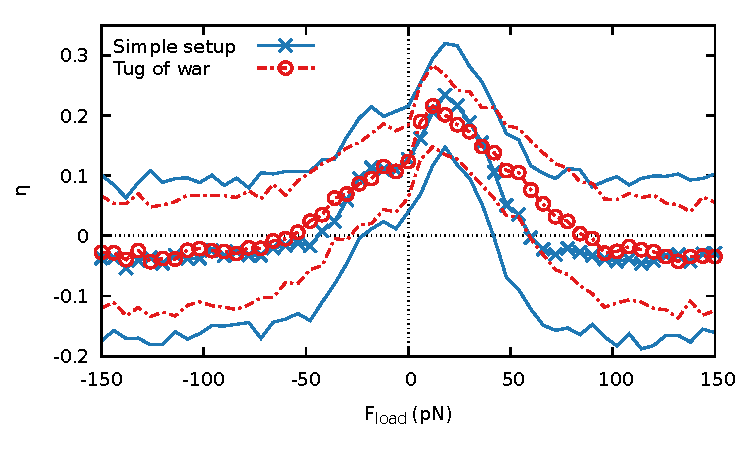
\includegraphics[width=.45\textwidth,height=!]{F_eta_setup.pdf}
\caption{\label{fig:load_efficiency_setups}
Comparison of the chemical efficiency~\eqref{eq:eta} as a function of the load $F_\text{load}$ for the ``load on the motor'', ``load on the polymer'' and the ``tug of war'' setups.
We observe that these efficiency profiles differ in the width of the distribution, while it's general shape remains the same.   
}
\end{figure}
The main difference between the curve for the ``load on the motor'' and ``load on the polymer'' setup is the width of the distribution. 
This can be understood from equations~\eqref{eq:chemical_excess} and~\eqref{eq:chemical_excess_poly}, 
where we see that the excess of the chemical energy entering the system is proportional to the relative velocity.
In the figure~\ref{fig:F_v_setups} we observe a different asymptotic behavior of the relative velocity by factor $\gamma_\text{M} / \gamma_\text{A}$,
hence we expect that the same factor applies in the steady state for the rate of the excess chemical heat production. 
This hypothesis is further confirmed in figure~\ref{fig:load_efficiency_setups_rescaled},
where we plot the chemical efficiency $\eta$ with respect to re-scaled load. 
\begin{figure}[t]
\centering
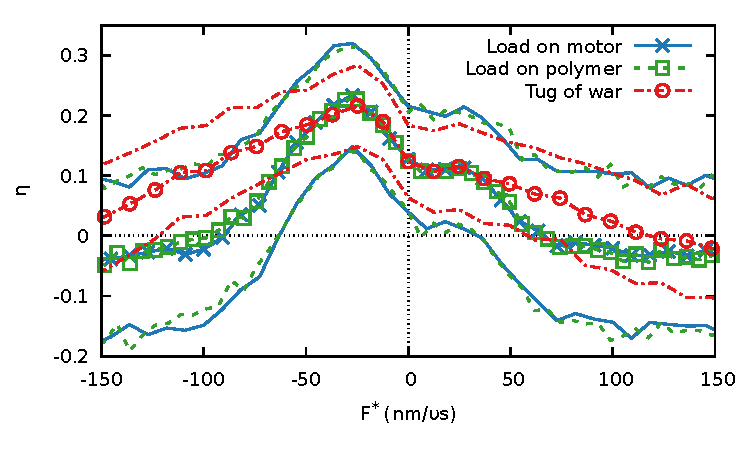
\includegraphics[width=.45\textwidth,height=!]{F_eta_setup_rescaled.pdf}
\caption{\label{fig:load_efficiency_setups_rescaled}
Comparison of the chemical efficiency~\eqref{eq:eta} as a function of the re-scaled load $F^*$ for the ``load on the motor'', ``load on the polymer'' and the ``tug of war'' setups.
For the ``load on the motor'' setup the re-scaled load is $F^* = F_\text{load} / \gamma_\text{M}$, 
while for the ``load on the polymer'' the re-scaled load is defined as $F^* = F_\text{load} / \gamma_\text{A}$.
Lastly, for the ``tug of war'' setup we define the re-scaled load as $F^* = 2 F_\text{load} / \gamma_\text{A}$,
where the factor $2$ comes from the fact that the load is applied once on each side of the system.
We observe that these efficiency profiles for ``load on the motor'' and ``load on the polymer'' collapse on each other.    
}
\end{figure}


\subsubsection{Tug of war}
Figures~\ref{fig:load_efficiency_setups} and~\ref{fig:load_efficiency_setups_rescaled} also depict the chemical efficiency $\eta$ dependency on the load $F_\text{load}$ for the ``tug of war'' setup, cf. section~\ref{sec:tug_of_war}.
We can see that the general shape is preserved.
In the figure~\ref{fig:load_efficiency_setups}, we can see that the large load asymptotic behavior correspond to the one of the ``load on the polymer'' setup.
This can be explained by the same asymptotic behavior for the relative velocity $\langle v\rangle$, cf. figure~\ref{fig:F_v_setups}, 
and for the tension on the motor $\tau_\text{M}$, cf. figure~\ref{fig:tug_F}, while having equation~\eqref{eq:excess_heat_tug} in mind.

For small loads, see figure~\ref{fig:load_efficiency_setups_rescaled}, the chemical efficiency for the ``tug of war'' setup corresponds to the ``load on polymer'' setup only when the load is scaled by a factor~$2$. 
This points to the fact that, rather then the external load $F_\text{load}$, the tension on the motor $\tau_\text{M}$ generated by the ratchet interaction is important,
which for small loads, when the polymer does not slip, is close to twice the external load. 
We will discuss this connection later, cf. figure~\ref{fig:tension_efficiency}. 


\subsubsection{Elastic environment}
In the case of elastic environment we observe, see figure~\ref{fig:stiffness_efficiency}, that the chemical efficiency~\eqref{eq:eta} is practically independent of the stiffness of the environment, $k_\text{sp}$. 
\begin{figure}[t]
\centering
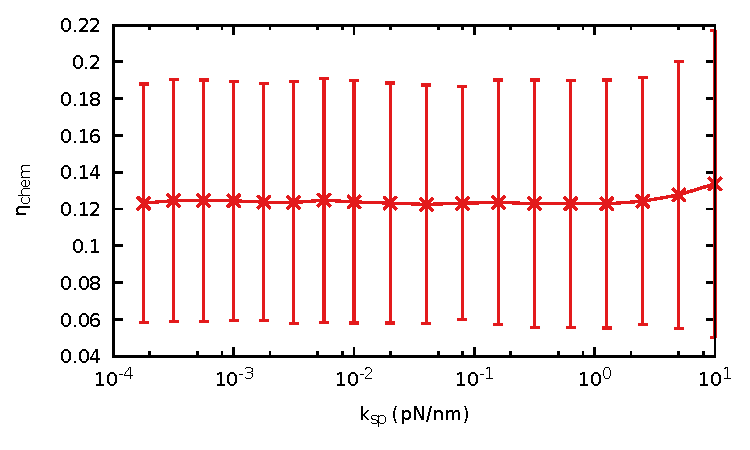
\includegraphics[width=.45\textwidth,height=!]{k_eta.pdf}
\caption{\label{fig:stiffness_efficiency}
The chemical efficiency~\eqref{eq:eta} as a function of the spring constant $k_\text{sp}$.
We observe a flat profile.
}
\end{figure}
Unfortunately, here we cannot use the same reasoning as for the ``tug of war'' setup, as the mean velocity of the motor in the steady state is zero. 

\subsubsection{Tension and chemical efficiency}
During the investigation of the chemical efficiency dependency on the external load $F_\text{load}$ for the ``tug of war'' setup, 
we discovered that rather than the load, the tension on the motor $\tau_\text{M}$ might be the intrinsic parameter. 
This is confirmed in the figure~\ref{fig:tension_efficiency}, 
where we plot the chemical efficiency as a function of the tension in the motor for all the setups mentioned above, 
and which represents our main result. 
\begin{figure}[t]
\centering
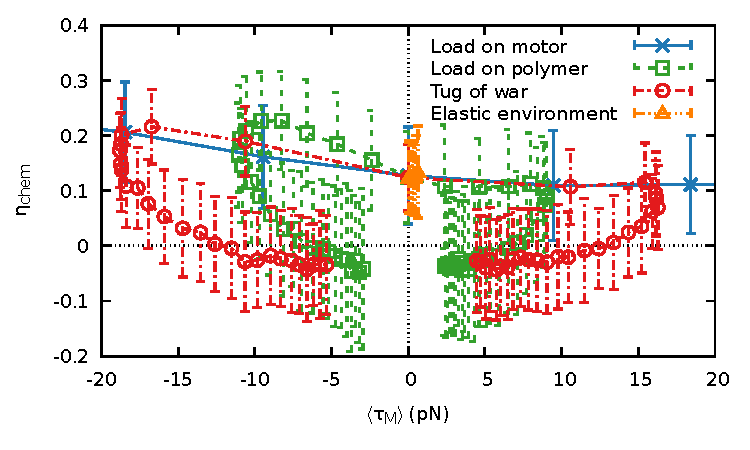
\includegraphics[width=.45\textwidth,height=!]{tension_eta.pdf}
\caption{\label{fig:tension_efficiency}
The chemical efficiency \eqref{eq:eta} as a function of the tension in the motor $\tau_\text{M}$.
%TODO
}
\end{figure}

For small tension, caused either by small external load $F_\text{load}$ or small stiffness of the surrounding network $k_\text{sp}$, 
the chemical efficiency has relatively flat profile with weak positive response to an increase in tension.
This can be explained by perturbations in the steady state average probability density for the motor's heads 
and was discussed in more details in the section~\ref{sec:chemical_efficiency}, 
cf. equations~\eqref{eq:eta} and~\eqref{eq:heat_flux_explicit}, and figures~\ref{fig:pos_distr} and~\ref{fig:chem_energy_distr}.  

With increasing load, both positive and negative, the tension on the motor in the ``load on the polymer'' and ``tug of war'' setups increase up to a certain threshold,
where the polymers start to slip with respect to the motor, and thus a further increase in the driving leads only to a decrease in the tension~\eqref{eq:tension_load_on_polymer_large} and~\eqref{eq:tension_tug}.
This creates a second branch of the dependency for the slipping motor, 
which is not present for the ``load on the motor'' setup, where there is always a residual tension from the load alone~\eqref{eq:tension_large_load}.  
For the ``tug of war'' setup the threshold value is larger than for the ``load on the polymer'' setup due to the interaction mediated by two ratchet potentials, one on each side of the polymer. 

These considerations complement the discussion that related the excess chemical energy with the build up tension in the motor, or more precisely with the additional tension created by the ratchet interaction, see discussion related to equations~\eqref{eq:chemical_excess_poly} and~\eqref{eq:excess_heat_tug}. 

Note that similar a discussion for the ``elastic environment'' setup is highly non-trivial, as shown in section~\ref{sec:power_elastic}.
However, the dependency of the efficiency on the tension follows a common pattern and fits the other results. 

In the end, we can conclude that the additional tension caused by the ratchet potential, in many models representing the tension in the motor itself, is the true intrinsic quantity which determines the chemical efficiency of the molecular motor. 


\section{Conclusions}
%TODO

With our proposed scaled-ratchet model we reproduce velocities and stall-forces of the myosin II molecular motor. 
These quantities depend heavily on the ATP binding rate $k_\text{bind}$.
We revisit the force-velocity relation for small non-muscle myosin II motors. 
We investigate how it depends on $k_\text{bind}$ and on the number of heads of the motor $N$.
In the ``load on the motor'' setup, mechanical quantities like the mean ratchet force and tension in the motor can be obtained by a linear combination of the mean relative velocity of the motor and the load applied to it. 
It is observed that for large loads, the motor begins to slip over the filament track and the force from the ratchet, and the tension generated by it, vanish.
The decay of the ratchet force corresponds to a theoretical result, obtained by a perturbative expansion around infinitely large loads.
Furthermore, the motor's ability of mechanosensing naturally emerges from the model without imposing a load-dependence on the chemical rates.
All dynamical aspects follow solely from the ratchet interaction between the motor and actin filament.
Lastly we define a chemical efficiency that quantifies the fraction of energy, supplied by ATP hydrolysis, 
that is consumed in the diffusion processes of the myosin II motor and actin filament.
This energy is partially used in the movement of the motor along the actin filament or in the build-up of tension in the motor, depending on the setup. 
The chemical efficiency is close to a local minimum when the motor is unloaded. 
When a load is applied, the ratchet force will counter the load and the chemical efficiency will increase. 
For large loads, the chemical efficiency decays and even becomes negative, which means that energy is drained from the diffusion process to the chemical cycle.

\begin{acknowledgments}
The authors are grateful to Christian Maes for many valuable discussions and to Bart Smeets and Maxim Cuvelier for proofreading of the manuscript.
\end{acknowledgments}

\appendix* 
\section{Perturbative treatment}
\label{sec:perturb}
Here we show that the chemical cycle must extract energy from the ratchet system with one head and for large load forces, 
i.e. the chemical efficiency \eqref{eq:eta} must be negative. 
We will show this by calculating the perturbative corrections to the probability density of the position of the motor with respect to the actin filament in the regime of large load $F_\text{load} \to \infty$, both in the ATP bound and ATP unbound state. 

First, we assume that the relaxation time of the position in a given potential is much shorter than the typical time between jumps in the chemical state of the heads. 
This effectively leads to time scale separations,
thus the conditional probability distribution \eqref{eq:cond_prob} is given as a steady state solution of the corresponding Fokker-Planck equation in a given state $\zeta$
\begin{multline*}
0 = \frac{1}{\gamma_\text{M}} \partial_\text{M} \left[ \left( F_\text{load} - \zeta \partial V_\text{r}( x_\text{M} - x_\text{A} ) \right) \mu\left( x_\text{M}, x_\text{A} \right)
\right. \\ \left.
- k_B T \partial_\text{M} \mu\left( x_\text{M}, x_\text{A} \right) \right] 
\\
+ \frac{1}{\gamma_\text{A}} \partial_\text{A} \left[ 
\zeta \partial V_\text{r} \mu( x_\text{M}, x_\text{A} ) 
- k_B T \partial_\text{A} \mu\left( x_\text{M}, x_\text{A} \right) 
\right] .
\end{multline*}
If we change the variables to describe the geometric center $x_C$ and the distance between motor and actin $\Delta x$
\begin{align*}
x_C &= \frac{1}{2} ( x_\text{M} + x_\text{A} ) , \\
\Delta x &= x_\text{M} - x_\text{A}, 
\end{align*}
a more convenient version of the Fokker-Planck is obtained
\begin{align*}
0 &= \begin{multlined}[t][.4\textwidth]
\partial_\Delta \Biggl[ 
\left( \frac{1}{\gamma_\text{M}} F_\text{load} - \left( \frac{1}{\gamma_\text{M}} + \frac{1}{\gamma_\text{A}} \right) \zeta \partial V_\text{r}( \Delta x ) \right) \mu
\\ 
- \left( \frac{1}{\gamma_\text{M}} + \frac{1}{\gamma_\text{A}} \right) k_B T \partial_\Delta \mu 
\Biggr] 
\end{multlined}
\\
&+ \begin{multlined}[t][.4\textwidth]
\frac{1}{2} \partial_C \Biggl[
\left( \frac{1}{\gamma_\text{M}} F_\text{load} - \left( \frac{1}{\gamma_\text{M}} - \frac{1}{\gamma_\text{A}} \right) \zeta \partial V_\text{r}( \Delta x ) \right) \mu
\\
- \frac{1}{2} \left( \frac{1}{\gamma_\text{M}} + \frac{1}{\gamma_\text{A}} \right) k_B T \partial_C \mu 
\Biggr] .
\end{multlined}
\end{align*}
If we integrate over all possible position of the center as our focus in this appendix is on the steady state distribution of the relative position of the motor and actin,
which completely determines the mean value of both the ratchet potential and the relative velocity, 
we obtain a reduced Fokker-Planck equation just for the aforementioned displacement ($x \equiv \Delta x$ further on)
\begin{equation}
0 = \frac{1}{\gamma^*} \partial_x \left[ \left( F^* - \zeta \partial_x V_\text{r}(x) \right) \rho(x) - k_B T \partial_x \rho(x) \right] ,
\label{eq:FP_ss}
\end{equation}
where $V_\text{r}$ is the ratchet potential \eqref{eq:ratchet_potential} and 
\begin{equation}
\begin{aligned}[.4\textwidth] 
\gamma^* &= \frac{ \gamma_\text{M} \gamma_\text{A} }{ \gamma_\text{M} + \gamma_\text{A} } , \\ 
F^* &= \frac{ \gamma_\text{A} }{ \gamma_\text{M} + \gamma_\text{A} } F_\text{load} . 
\end{aligned} 
\label{eq:rescale_parameters}
\end{equation}

The first step is expressing the equation \eqref{eq:FP_ss} in terms of $\epsilon = ( F^* )^{-1}$ instead of load force $f_\text{load}$,
which makes it more convenient for the expansion
\begin{equation}
\partial_x \left[ \rho(x) - \epsilon \left( \zeta \partial_x V_\text{r}(x) \rho(x) + k_B T \partial_x \rho(x) \right) \right] = 0 
\label{eq:FP_ss_pert}
\end{equation}
Due to the periodical boundary conditions, the zeroth order approximation correspond to the flat distribution, i.e. $\rho_0 = \frac{1}{\ell}$. 
Note that at the leading order the conditional probability density is independent of the internal state $\zeta$,
thus the chemical efficiency \eqref{eq:eta} is zero. 

For the first order solution we start with an ansatz $\rho_1 = \rho_0 + \delta\rho_1$. 
When inserted into \eqref{eq:FP_ss_pert} we get
\begin{equation*}
\delta\rho_1 = \frac{\epsilon}{\ell} \partial_x V_\text{r} + C
\end{equation*}
where $C$ is an integration constant.
Due to the normalization 
\begin{equation}
1 = \int\limits_0^\ell \rmd x \; \rho_1(x), 
\label{eq:normalization}
\end{equation}
and periodicity of the ratchet potential \eqref{eq:ratchet_potential} the aforementioned integration constant has to be equal to $0$.

Note, that the first order correction does not contribute to calculations of $\langle V_\text{r} | \zeta \rangle_\rho$ 
\begin{multline*}
\langle V_\text{r} | \zeta \rangle_{\delta \rho_1} 
= \int\limits_0^\ell V_\text{r}(x) \, \delta\rho_1(x) \; \rmd x
\\
\propto \int\limits_0^\ell V_\text{r}(x) \, \partial_x V_\text{r}(x) \; \rmd x 
= \frac{1}{2} \int\limits_0^\ell \partial_x V_\text{r}^2(x) \; \rmd x 
= 0
\end{multline*}
where we again used the fact that the ratchet potential $V_\text{r}(x)$ is periodic.

Consequently, we need to calculate the second order correction $\delta\rho_2$. 
Starting from the ansatz $\rho_2 = \rho_1 + \delta\rho_2$ in \eqref{eq:FP_ss_pert} and keeping up the terms up to quadratic order in $\epsilon$, we find
\begin{equation*}
\delta\rho_2 = \frac{ \epsilon^2 }{ \ell } \left[ \left( \zeta \partial_x V_\text{r} \right)^2 - k_B T \zeta \partial_x^2 V_\text{r} \right] + C^\prime .
\end{equation*}
Again by requiring the normalization~\eqref{eq:normalization}, the integration constant $C^\prime$ can be determined
\begin{multline*}
1 = \int\limits_0^\ell \rho_2(x) \; \rmd x 
\\
= 1  
+ \frac{\epsilon^2}{ \ell } \int\limits_0^\ell \left[ \left( \zeta \partial_x V_\text{r}(x) \right)^2 - k_B T \zeta \partial_x^2 V_\text{r}(x) \right] \; \rmd x 
+ \ell C^\prime ,
\end{multline*}
which leads to
\begin{equation}
C^\prime = - \frac{\epsilon^2 \zeta^2}{ \ell^2 } \int\limits_0^\ell \left( \partial_x V_\text{r}(x) \right)^2 \; \rmd x . 
\end{equation}
Now the density up to second order is given by
\begin{multline}
\rho_2(x)  
= \frac{1}{\ell} \Biggl\{ 1  + \epsilon \zeta \partial_x V_\text{r}(x) \\
+ \epsilon^2 \zeta^2 \left[ \left( \partial_x V_\text{r}(x) \right)^2 - \frac{1}{\ell} \int\limits_0^\ell \left( \partial_y V_\text{r}(y) \right)^2 \; \rmd y \right] 
\\
- \epsilon^2 \zeta k_B T \partial_x^2 V_\text{r}(x)  
\Biggr\} .
\label{eq:prob_density_large}
\end{multline}
Note that up to the quadratic order in $\epsilon$ the conditional probability density depends on the ratchet potential only through a first or second order derivatives. 
Therefore the density will appear as a piece-wise constant function on $x \in [0,\ell]$, with different values for $x < a \ell$ and $x > a \ell$. 
This trend can already be seen in the empirical density obtained from simulations for large load forces $F^* = \pm 250 \, \mathrm{pN}$ in figure~\ref{fig:pos_distr},
and is further demonstrated on motor with a single head in figure~\ref{fig:prob_density_large}. 
\begin{figure}[t]
\centering
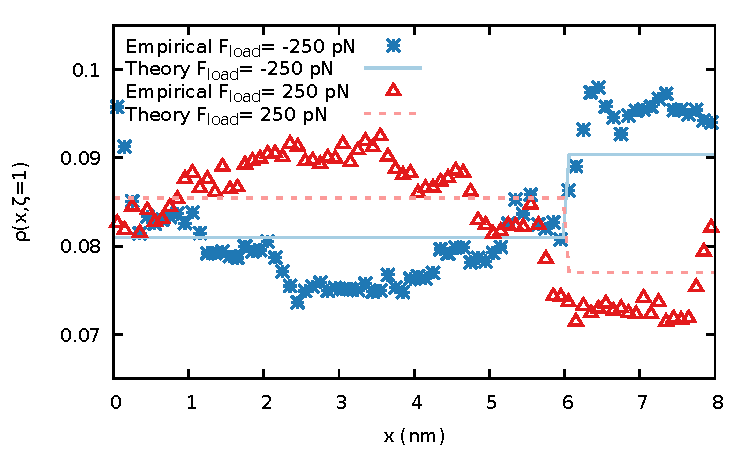
\includegraphics[width=0.45\textwidth,height=!]{pos_compare.pdf}
\caption{\label{fig:prob_density_large}
Empirical probability density for large loads for motor with single head in an ATP unbound state compared with the theoretical prediction \eqref{eq:prob_density_large}.
}
\end{figure}
%\begin{figure*}[t]
%\centering
%\subfigure[Positive load]{
%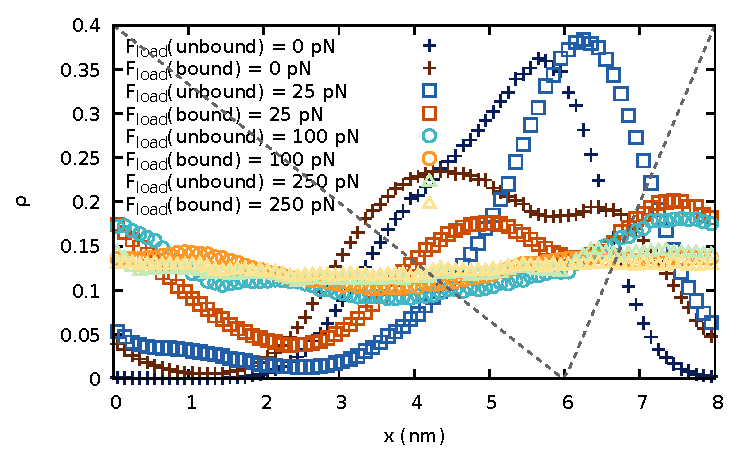
\includegraphics[width=0.45\textwidth,height=!]{pos_multiplot_p}
%}
%\subfigure[Negative load]{
%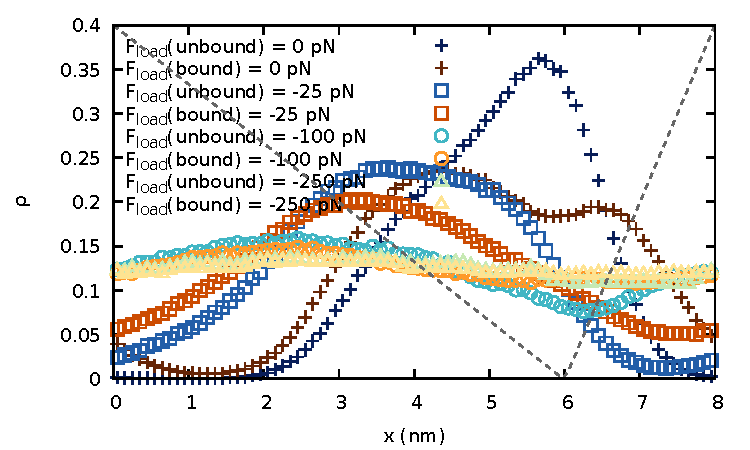
\includegraphics[width=0.45\textwidth,height=!]{pos_multiplot_m}
%}
%\caption{
%\label{fig:pos_multiplot}
%Side by side comparison of empirical density profiles in both attachable (a - blue colored) and detached (d - red colored) state for different loads.
%Profiles sharing the same load magnitude $|F^*|$ are denoted by the symbols.
%}
%\end{figure*}


With the second order correction, we can now calculate the change in the expected value of the potential energy
\begin{align*}
\langle V_\text{r} | \zeta \rangle_{\delta\rho_2} 
=& \int\limits_0^\ell V_\text{r}(x) \, \delta\rho_2 \; \rmd x \\
=& \frac{\epsilon^2 \zeta^2}{\ell} \int\limits_0^\ell V_\text{r}(x) \left(\partial_x V_\text{r}(x) \right)^2 \; \rmd x  \\
&- \frac{\epsilon^2 \zeta^2}{\ell^2} \int\limits_0^\ell V_\text{r}(x) \; \rmd x \int\limits_0^\ell \left( \partial_y V_\text{r}(y) \right)^2 \; \rmd y \\
&- \frac{\epsilon^2 \zeta k_B T}{\ell} \int\limits_0^\ell V_\text{r}(x) \, \partial_x^2 V_\text{r}(x) \; \rmd x .
\end{align*}
After tedious but straightforward calculation we found that the first two terms will cancel each other. 
Hence only the last term remains, which after an explicit calculation leads to  
\begin{align*}
\langle V_\text{r} | \zeta = 1 \rangle_{\rho_2} &= \frac{V}{2} + \frac{k_B T}{(F^*)^2} \frac{V^2}{a \left(1-a\right) \ell^2 }, \\
\langle V_\text{r} | \zeta = c \rangle_{\rho_2} &= \frac{V}{2} + \frac{k_B T}{(F^*)^2} \frac{c V^2}{a \left(1-a\right) \ell^2 } .
\end{align*}
By using these expression we get the chemical efficiency~\eqref{eq:eta} up to the second order in $\epsilon$  
\begin{align*}
\eta_\text{chem} 
&= - \frac{ \left(1-c\right)^2 }{ a (1-a) } \, \frac{k_B T} { \Delta E - (1-c) \frac{V}{2} } \left( \frac{V}{\ell F^*} \right)^2 
\\
&= - \frac{ \left(1-c\right)^2 }{ a (1-a) } 
\frac{k_B T} { \Delta E - (1-c) \frac{V}{2} } 
\left[ \frac{ ( \gamma_\text{A} + \gamma_\text{M} ) V }{\gamma_\text{A} \ell F_\text{load}} \right]^2 .
\end{align*}
As was advertised, the zeroth and linear order in $\epsilon$ do not contribute, 
the chemical efficiency decays towards zero as $F_\text{load}^{-2}$ and it is negative for large loads independently of the direction of the load.
The symmetry for of the chemical efficiency $\eta_\text{chem}$ is for large loads confirmed in the figure~\ref{fig:chem}. 
The fact that the chemical efficiency is negative in this regime, 
means the driven system builds up a chemical energy in the environment, while the external force is performing work on the system. 
Also note that in the expression for the chemical efficiency, 
the ratio between the amplitude of the ratchet potential $V$ and the work done by the external force over a period of the potential $\ell F^*$ appears in the formula, 
as well as the ratio between the thermal energy $k_B T$ and the mean energy gap between the attached and detached state. 

In addition we can compute the steady state probabilistic current in each respective internal state.
The probabilistic current is given by 
\[
\mathcal{J}(x) = \frac{1}{\gamma^*} \left[ \left( F^* - \partial_x V_\text{r}(x) \right) \rho(x) - k_B T \partial_x \rho(x) \right] 
\]
Which simplifies in the second order in the large load regime to
\begin{align*}
\mathcal{J}(x) 
&= \frac{F^*}{\gamma^* \ell} - \frac{\zeta^2}{F^* \gamma^* \ell^2} \int\limits^\ell_0 \left( \partial_x V_\text{r}(x) \right)^2 \; \rmd x \\
&= \frac{F^*}{\gamma^* \ell} - \frac{\zeta^2 V^2}{\gamma^* F^* \ell^3 a (1-a) } ,
\end{align*}
which is independent of the position. 
Note, that the current integrated over the period of the ratchet $\ell$, represents the mean velocity of the motor in the given state
\begin{multline}
\left\langle v \middle| \zeta \right\rangle 
= \int\limits_0^\ell \rmd x \; {\mathcal J}(x) 
= \frac{F^*}{\gamma^*} - \frac{\zeta^2 V^2}{\gamma^* F^* \ell^2 a (1-a) } 
\\
= \frac{F_\text{load}}{\gamma_\text{M}} - \frac{ ( \gamma_\text{M} + \gamma_\text{A} ) \zeta^2 V^2}{\gamma_\text{M} \gamma_\text{A} F_\text{load} \ell^2 a (1-a) } .
\label{eq:mean_velocity_large}
\end{multline}
Indeed, the dominant term for large external forces is $\langle v \rangle_{\rho_0} = F_\text{load} / \gamma_\text{M}$ independently of the internal state, 
which was already demonstrated in the figure~\ref{fig:F_v}. 
Furthermore, the force-independent term (i.e. term proportional to $F_\text{load}^0$) vanishes leading to an anti-symmetric form with respect to the load $F_\text{load}$. 
The first correction decay linearly in the external load, which was clearly seen in the figure~\ref{fig:ratchet_force_decay}, 
which exposes the first correction to the mean velocity, cf. equation~\eqref{eq:mean_ratchet_force}. 
As there is no fundamental difference in the Fokker-Planck equation for one head and for four heads regarding the currents for large driving forces, 
the result obtained for a one-headed motor also holds for the simulations of motors with four heads. 

\bibliography{ratchet}


\end{document}
